%%%%%%%%%%%%%%%%%%%%%%%%%%%%%%%%%%%%%%%%%%%%%%%%%%%%%%%%%%%%%%%%%%%%%%
% Lớp 10 | Mệnh đề. Tập hợp | Tập hợp
% Dạng 0D1?2-2: Tập hợp con. Hai tập hợp bằng nhau
% Số câu: 149  (sinh tự động bởi tach_cau.py; từ nay thầy sửa trực tiếp file này)
%%%%%%%%%%%%%%%%%%%%%%%%%%%%%%%%%%%%%%%%%%%%%%%%%%%%%%%%%%%%%%%%%%%%%%

%%%%%%%%%%%%%%%% TRẮC NGHIỆM 4 PHƯƠNG ÁN %%%%%%%%%%%%%%%%

% nguồn: MaHoaNH_TracNghiem_Lop10
\begin{ex}%[0D1N2-2]%[ma:901ef3a5]
	Cho tập hợp $A=\{0;2;4;8\}$. Số tập hợp con gồm hai phần  tử của $A$ là
	\choice { $12$}{ $4$}{ $8$}{\True  $6$}
	\loigiai{ 
		Số tập hợp con gồm hai phần  tử của A là số cách chọn 2 phần tử từ 4 phần tử, tức là $\mathrm{C}_{4}^{2}=6$.\\
		Các tập hợp đó là $\{0;2\},\{0;4\},\{0;8\},\{2;4\},\{2;8\},\{4;8\}$. 
	} 
\end{ex}

% nguồn: MaHoaNH_TracNghiem_Lop10
\begin{ex}%[0D1N2-2]%[ma:3edc5511]
	 Tập hợp nào sau đây là tập hợp con của tập hợp $\mathbb{Z}$?
	\choice 
		{$\left\{\sqrt{2};3;4\right\}$} 
		{$\left\{\dfrac{1}{3};5;-3\right\}$} 
		{\True $\left\{-1;0;1\right\}$} 
		{$\left\{\pi;2;-4\right\}$} 
	 \loigiai{
	Ta có $-1\in\mathbb{Z}$,  $0\in\mathbb{Z}$, $1\in\mathbb{Z}$ nên $\left\{-1;0;1\right\}$ là tập con của tập hợp $\mathbb{Z}$.}
\end{ex}

% nguồn: MaHoaNH_TracNghiem_Lop10
\begin{ex}%[0D1N2-2]%[ma:a31cd0d0]
	Cho tập hợp $X=\{0; 2; 5\}$. Tập hợp nào dưới  đây $\textbf{không}$ phải là tập con của tập hợp $X$?
	\choice 
		{$\varnothing$} 
		 {$\{2\}$}
		{$\{0;  2; 5\}$}
		{\True $\{0; 1; 2\}$} 
	\loigiai{ 
		Ta  có $1 \notin X$, vậy $\{0; 1; 2\} \not \subset\{0; 2; 5\}$.
	} 
\end{ex}

% nguồn: MaHoaNH_TracNghiem_Lop10
\begin{ex}%[0D1N2-2]%[ma:282d55a8]
	Số phần tử của tập $C=\{x  \in \mathbb{Z} \mid-1 \leqslant x \leqslant 1\}$ là
	\choice 
		{\True  $3$}
		 {$2$}
		{$1$} 
		{$6$} 
	\loigiai{ 
		Ta có $C=\{-1; 0; 1\}$ nên $C$ có $3$ phần tử. 
	 }
\end{ex}

% nguồn: MaHoaNH_TracNghiem_Lop10
\begin{ex}%[0D1H2-2]%[ma:7e029506]
	Cho tập hợp $A=\left\{1; 2; a\right\}$, $B=\left\{1; 2; a; b; x; y\right\}$. Hỏi có bao nhiêu tập  hợp $X$ thỏa $A\subset X\subset B$?
	\choice 
		{\True $8$} 
		{$7$} 
		{$6$} 
		 {$2^n$}
	\loigiai{Các tập hợp $X$ thoả là $\left\{1; 2; a\right\}$, $\left\{1; 2; a;b\right\}$, $\left\{1; 2; a;x\right\}$, $\left\{1; 2; a; y\right\}$,  $\left\{1; 2; a;b;x\right\}$, $\left\{1; 2; a;b;y\right\}$, $\left\{1; 2; a;x;y\right\}$, $\left\{1; 2; a; b; x; y\right\}$.}
\end{ex}

% nguồn: MaHoaNH_TracNghiem_Lop10
\begin{ex}%[0D1H2-2]%[ma:27463cd0]
	Trong các mệnh đề sau đây, mệnh  đề nào \textbf{sai}?
	\choice 
		 {$A\subset A$}
		 {$\varnothing \subset A$}
		{$A\in  \varnothing$}
		{$\varnothing \subset \varnothing$} 
	\loigiai{Mệnh đề sai là $A\in  \varnothing$.}
\end{ex}

% nguồn: MaHoaNH_TracNghiem_Lop10
\begin{ex}%[0D1H2-2]%[ma:befb22f7]
	Tập hợp  nào sau đây có đúng hai tập hợp con?
	\choice 
		 {$\left\{x;\varnothing \right\}$}
		 {\True $\{x\}$}
		 {$\left\{x;y;\varnothing \right\}$}
		{$\left\{x;y\right\}$} 
	\loigiai{Công thức số tập con của tập hợp có $n$  phần tử là $2^n$ nên suy ra tập $\{x\}$ có $1$ phần tử nên có $2^1=2$ tập con.}
\end{ex}

% nguồn: MaHoaNH_TracNghiem_Lop10
\begin{ex}%[0D1H2-2]%[ma:8dc4028f]
	Cho tập hợp $A=\left\{0;3;4;6\right\}$. Số tập hợp con gồm hai phần tử của  $A$ là
	\choice 
		{$12$} 
		{$8$} 
		 {$10$}
		{\True $6$} 
	\loigiai{Mỗi tập con gồm hai phần tử của $A$ là $\left\{0;3;\right\}$, $\left\{0;4\right\}$, $\left\{0;6\right\}$, $\left\{3;4\right\}$, $\left\{3;6\right\}$,  $\left\{4;6\right\}$.}
\end{ex}

% nguồn: MaHoaNH_TracNghiem_Lop10
\begin{ex}%[0D1H2-2]%[ma:58a43af1]
	Trong các tập hợp sau đây,  tập hợp nào có đúng một tập hợp con?
	\choice 
		{\True $\varnothing$} 
		{$\{x\}$} 
		{$\left\{\varnothing  \right\}$}
		{$\left\{\varnothing,  x\right\}$}
	\loigiai{Vì tập $\varnothing$ có  tập hợp con là chính nó.
	 }
\end{ex}

% nguồn: MaHoaNH_TracNghiem_Lop10
\begin{ex}%[0D1H2-2]%[ma:6b4bfa60]
	Trong các tập hợp sau đây,  tập hợp nào có đúng hai tập hợp con?
	 \choice
		{$\left\{x;y\right\}$} 
		 {\True $\{x\}$}
		 {$\left\{\varnothing;x\right\}$}
		{$\left\{\varnothing;x;y\right\}$} 
	\loigiai{Vì tập hợp $\{x\}$ có hai tập con là $\varnothing$ và chính  nó.
	} 
\end{ex}

% nguồn: MaHoaNH_TracNghiem_Lop10
\begin{ex}%[0D1H2-2]%[ma:9780720b]
	Cho hai tập  hợp $X=\{n\in \mathbb{N}\mid n \text{ là bội số của $4$ và $6$ }\}$ và $Y=\{n\in \mathbb{N}\mid n \text{ là bội số của $12$ }\}$. Trong các mệnh đề sau, tìm mệnh đề \textbf{sai}?
	 \choice
		 {$X\subset Y$}
		{$Y\subset  X$}
		{\True  $X=Y$}
		{$\exists n\mid  n\in X$ và $n\notin Y$}
	 \loigiai{Vì bội số chung nhỏ nhất của $4$ và $6$ là $12$.
	} 
\end{ex}

% nguồn: MaHoaNH_TracNghiem_Lop10
\begin{ex}%[0D1H2-2]%[ma:49abf733]
	Cách viết nào sau đây  là đúng?
	 \choice
		{$a\subset \left[a;b\right]$} 
		{\True $\{a\}\subset \left[a;b\right]$} 
		{$\{a\}\in \left[a;b\right]$} 
		 {$a\in \left(a;b\right]$}
	 \loigiai{Cách viết đúng là $\{a\}\subset \left[a;b\right]$.
	 }
\end{ex}

% nguồn: MaHoaNH_TracNghiem_Lop10
\begin{ex}%[0D1H2-2]%[ma:c54d5d1c]
	Cho tập hợp $P$. Tìm mệnh đề \textbf{sai} trong các mệnh đề sau? 
	\choice 
		{$P\subset P$} 
		 {$\varnothing \subset P$}
		{$P\in \left\{P\right\}$} 
		 {\True $P\in P$}
	\loigiai{Mệnh  đề sai là $P\in P$.
	} 
\end{ex}

% nguồn: MaHoaNH_TracNghiem_Lop10
\begin{ex}%[0D1H2-2]%[ma:894f0e6a]
	Số tập con của tập hợp có  $n$ ($n\ge 1$, $n\in \mathbb{N}$) phần tử là
	\choice 
		 {$2^{n+2}$}
		 {$2^{n-1}$}
		 {$2^{n+1}$}
		{\True  $2^n$}
	\loigiai{Số tập con của tập hợp  có $n$ bằng $2^n$.
	} 
\end{ex}

% nguồn: MaHoaNH_TracNghiem_Lop10
\begin{ex}%[0D1H2-2]%[ma:9bc538b0]
	Cho tập hợp $A=\left\{1;2;3;4\right\}$, $B=\left\{0;2;4\right\}$, $C=\left\{0;1;2;3;4;5\right\}$. Quan hệ  nào sau đây là đúng?
	\choice 
		{$B\subset A\subset  C$}
		 {$B\subset A=C$}
		{\True $\heva{&A\subset  C\\&B\subset C}$}
		 {$A\cup B=C$}
	\loigiai{Ta thấy mọi phần  tử của $A$ đều thuộc $C$ và mọi phần tử của $B$ đều thuộc $C$.
	 }
\end{ex}

% nguồn: MaHoaNH_TracNghiem_Lop10
\begin{ex}%[0D1H2-2]%[ma:b085fcd1]
	Cho  tập hợp $A$. Trong các mệnh đề sau, mệnh đề nào \textbf{sai}?
	\choice 
		{$\varnothing \subset A$} 
		{$A\ne  \left\{A\right\}$}
		{\True  $A\in A$}
		{$A\subset A$} 
	\loigiai{Mệnh đề sai  là $A\in A$.
	 }
\end{ex}

% nguồn: MaHoaNH_TracNghiem_Lop10
\begin{ex}%[0D1H2-2]%[ma:49bda3d4]
	Số các tập  hợp con có $3$ phần tử có chứa $a$, $b$ của tập hợp $C=\left\{a;b;c;d;e;f;g\right\}$ là
	 \choice
		{\True $5$} 
		 {$6$}
		{$7$} 
		{$8$} 
	\loigiai{Tập con có  $3$ phần tử trong đó $a$, $b$ luôn có mặt.\\
		Vậy phần tử thứ $3$ sẽ thuộc một trong các phần tử $c$, $d$, $e$, $f$, $g$ ($5$ phần tử)  nên có $5$ tập con.
	} 
\end{ex}

% nguồn: MaHoaNH_TracNghiem_Lop10
\begin{ex}%[0D1H2-2]%[ma:a11d9926]
	Cho tập hợp $A$ có $4$ phần tử. Hỏi tập $A$ có bao nhiêu tập con  khác rỗng?
	 \choice
		{$16$} 
		{\True  $15$}
		{$12$} 
		 {$7$}
	\loigiai{Vì số tập con của tập $4$ phần tử  là $2^4=16$.\\
		Suy ra  số tập con khác rỗng là $16-1=15$.
	} 
\end{ex}

% nguồn: MaHoaNH_TracNghiem_Lop10
\begin{ex}%[0D1H2-2]%[ma:47f29e4f]
	Cho tập  hợp $A=\left\{x^2+1\mid x\in \mathbb{N}^{*},\ x^2\le 5\right\}$. Khi đó tập $A$ bằng tập hợp nào sau đây?
	 \choice
		 {$A=\left\{1;2;3;4\right\}$}
		 {$A=\left\{0;2;5\right\}$}
		{\True $A=\left\{2;5\right\}$} 
		 {$A=\left\{0;1;2;3;4;5\right\}$}
	\loigiai{Ta có $\heva{&x^2\le 5 \\&x\in \mathbb{N^*}} \Leftrightarrow \heva{&-\sqrt{5} \le x\le \sqrt{5} \\  &x\in \mathbb{N^*}} \Leftrightarrow x\in \left\{1;2\right\}\Rightarrow \left(x^2+1\right)\in \left\{2;5\right\}$.\\
		 Vậy $A=\left\{2;5\right\}$.
	} 
\end{ex}

% nguồn: MaHoaNH_TracNghiem_Lop10
\begin{ex}%[0D1H2-2]%[ma:7ce91644]
	Cho tập hợp  $A=\left\{1;3\right\},B=\left\{3;x\right\},C=\left\{x;y;3\right\}$. Để $A=B=C$ thì tất cả các cặp $\left(x;y\right)$ là
	\choice 
		 {$\left(1;1\right)$}
		{\True $\left(1;1\right)$ và $\left(1;3\right)$} 
		{$\left(1;3\right)$} 
		{$\left(3;1\right)$ và  $\left(3;3\right)$}
	\loigiai{Ta có $A=B=C\Leftrightarrow \heva{&x=1\\&\hoac{&{y=1} \\&{y=3.}}}$\\ 
		Suy ra cặp $\left(x;y\right)$ là $\left(1;1\right);\left(1;3\right)$. 
	} 
\end{ex}

% nguồn: MaHoaNH_TracNghiem_Lop10
\begin{ex}%[0D1H2-2]%[ma:94adee0e]
	Số các tập con $2$ phần tử của $B=\left\{a,b,c,d,e,f\right\}$  là
	 \choice
		{\True  $15$}
		 {$16$}
		{$22$} 
		{$25$} 
	\loigiai{ 
		Số  các tập con $2$ phần tử của $B=\left\{a,b,c,d,e,f\right\}$ là $\mathrm{C}_6^2=15$ (sử dụng máy tính bỏ túi).
	} 
\end{ex}

% nguồn: MaHoaNH_TracNghiem_Lop10
\begin{ex}%[0D1H2-2]%[ma:c26e1bb6]
	Cho  tập hợp $A=\left\{a,b,c,d\right\}$. Tập $A$ có mấy tập con?
	 \choice
		{\True  $16$}
		 {$15$}
		{$12$} 
		 {$10$}
	\loigiai{ 
		Số tập con của tập  $A$ là $2^4=16$.
	} 
\end{ex}

% nguồn: MaHoaNH_TracNghiem_Lop10
\begin{ex}%[0D1H2-2]%[ma:a911c141]
	Hai tập hợp nào dưới  đây \textbf{không} bằng nhau?
	 \choice
		{\True $A=\left\{x\mid x=\dfrac{1}{2^k}, k\in \mathbb{Z},x\ge \dfrac{1}{8}  \right\}$ và $B=\left\{\dfrac{1}{2};\dfrac{1}{4};\dfrac{1}{8} \right\}$}
		{$A=\left\{3;9;27;81\right\}$ và $B=\left\{3^n\mid  n\in \mathbb{N},1\le n\le 4\right\}$}
		{$A=\left\{x\in \mathbb{Z}\mid -2< x\le 3\right\}$ và  $B=\left\{-1;0;1;2;3\right\}$}
		{$A=\left\{x\in \mathbb{N}\mid x <  5\right\}$ và $B=\left\{0;\; 1;\; 2;\; 3;\; 4\right\}$}
	\loigiai{Xét tập hợp $A=\left\{x\mid x=\dfrac{1}{2^k}, k\in \mathbb{Z},x\ge \dfrac{1}{8} \right\}$,\\ Ta có $\dfrac{1}{2^k} \ge \dfrac{1}{8} \Leftrightarrow \dfrac{1}{2^k} \ge \dfrac{1}{2^3} \Leftrightarrow 2^k \le 2^3\Leftrightarrow  k\le 3$.\\
		Suy ra $A=\left\{x\mid x=\dfrac{1}{2^k}, k\in \mathbb{Z},k\le 3\right\}$ $\Leftrightarrow A=\left\{\dfrac{1}{8};\dfrac{1}{4};\dfrac{1}{2};\ldots \right\}$  nên $A\ne B$.
	 }
\end{ex}

% nguồn: MaHoaNH_TracNghiem_Lop10
\begin{ex}%[0D1H2-2]%[ma:308ff1cb]
	Cho tập hợp $A=\left\{1;2\right\}$ và $B=\left\{1;2;3;4;5\right\}$. Có tất cả bao nhiêu tập $X$  thỏa mãn $A\subset X\subset B$?
	\choice 
		 {$5$}
		 {$6$}
		 {$7$}
		{\True $8$} 
	\loigiai{$X$ là tập hợp phải luôn  có mặt $1$ và $2$.\\
		Vì vậy ta đi tìm số tập con của tập $\left\{3;4;5\right\}$, sau đó cho hai phần tử $1$ và  $2$ vào các tập con nói trên ta được tập $X$.\\
		Vì số tập con của tập $\left\{3;4;5\right\}$ là $2^3=8$  nên có $8$ tập $X$.
	 }
\end{ex}

% nguồn: MaHoaNH_TracNghiem_Lop10
\begin{ex}%[0D1H2-2]%[ma:12259bc3]
	Cho tập hợp $A=\left\{1,2,3,4,x,y\right\}$. Xét các mệnh  đề sau đây (I): \lq\lq $3\in A$\rq\rq. (II): \lq\lq $\left\{3,4\right\}\in A$\rq\rq. (III): \lq\lq $\left\{a,3,b\right\}\in A $\rq\rq. Trong các mệnh đề sau, mệnh đề nào đúng
	 \choice
		{\True $I$ đúng} 
		 {$I$, $II$ đúng}
		 {$II$, $III$ đúng}
		 {$I$, $III$ đúng}
	\loigiai{$3$ là  một phần tử của tập hợp $A$.\\
		$\left\{3,4\right\}$ là một tập con của tập hợp $A$. Ký  hiệu $\left\{3,4\right\}\subset A$.\\
		 $\left\{a,3,b\right\}$ là một tập con của tập hợp $A$. Ký hiệu $\left\{a,3,b\right\}\subset A$.
	} 
\end{ex}

% nguồn: MaHoaNH_TracNghiem_Lop10
\begin{ex}%[0D1H2-2]%[ma:feed07e2]
	Số các tập hợp con gồm hai phần tử của  tập hợp $B=\left\{a;b;c;d;e;f\right\}$ là
	\choice 
		{\True $15$} 
		{$16$} 
		{$22$} 
		{$25$} 
	\loigiai{Số tập con có  $2$ phần tử trong đó có phần tử $a$ là $5$ tập gồm $\left\{a;b\right\}$, $\left\{a;c\right\}$, $\left\{a;d\right\}$, $\left\{a;e\right\}$, $\left\{a,f\right\}$.\\
		Số tập con có $2$ phần tử mà luôn có phần  tử $b$ nhưng không có phần tử $a$ là $4$ tập gồm $\left\{b;c\right\}$, $\left\{b;d\right\}$, $\left\{b;e\right\}$, $\left\{b;f\right\}$.\\
		 Tương tự ta có tất cả $5+4+3+2+1=15$ tập.
	 }
\end{ex}

% nguồn: MaHoaNH_TracNghiem_Lop10
\begin{ex}%[0D1H2-2]%[ma:0829baf9]
	Số các tập con $3$ phần tử có chứa $\alpha, \pi$ của $C=\left\{\alpha,  \; \pi, \; \xi, \; \psi, \; \rho, \; \eta, \; \gamma, \; \sigma, \; \omega, \; \tau \right\}$ là
	\choice 
		 {\True $8$}
		 {$10$}
		 {$12$}
		{$14$} 
	\loigiai{ 
		Các tập con $3$ phần tử có chứa $\alpha, \pi$ của $C=\left\{\alpha, \; \pi,  \; \xi, \; \psi, \; \rho, \; \eta, \; \gamma, \; \sigma, \; \omega, \; \tau \right\}$ là
		\[\left\{\alpha, \pi, \xi \right\}, \left\{\alpha, \pi, \psi \right\}, \left\{\alpha, \pi, \rho \right\}, \left\{\alpha, \pi, \eta  \right\}, \left\{\alpha, \pi, \gamma \right\}, \left\{\alpha, \pi, \sigma \right\}, \left\{\alpha, \pi, \omega \right\}, \left\{\alpha, \pi, \tau \right\}.\]
	} 
\end{ex}

% nguồn: MaHoaNH_TracNghiem_Lop10
\begin{ex}%[0D1H2-2]%[ma:f72f5f06]
	Cho  tập hợp $X=\left\{a;b;c\right\}$. Số tập con của $X$ là
	 \choice
		 {$4$}
		 {$6$}
		{\True  $8$}
		{$12$} 
	\loigiai{Số tập con không có phần tử nào  là $1$ (tập $\varnothing$).\\
		Số tập con có $1$ phần tử là  $3$ tập hợp $\{a\}$, $\{b\}$, $\{c\}$.\\
		Số tập con có $2$ phần tử là $3$ tập hợp $\left\{a;b\right\}$, $\left\{a;c\right\}$,  $\left\{b;c\right\}$.\\
		Số tập  con có $3$ phần tử là $1$ tập hợp $\left\{a;b;c\right\}$. \
		Vậy  có $1+3+3+1=8$ tập con.
	 }
\end{ex}

% nguồn: MaHoaNH_TracNghiem_Lop10
\begin{ex}%[0D1H2-2]%[ma:ae67f744]
	Trong các tập sau đây, tập hợp nào  có đúng hai tập hợp con?
	 \choice
		{$\left\{x;y\right\}$} 
		{\True $\{x\}$} 
		{$\left\{\varnothing;x\right\}$} 
		{$\left\{\varnothing;x;y\right\}$} 
	 \loigiai{
		\begin{itemize}
			\item $\left\{x;y\right\}$  có $2^2=4$ tập con.
			\item $\{x\}$  có $2^1=2$ tập con là $\{x\}$ và $\varnothing$.
			\item $\left\{\varnothing;x\right\}$  có $2^2=4$ tập con.
			\item $\left\{\varnothing;x;y\right\}$ có $2^3=8$ tập con. 
		\end{itemize}
	} 
\end{ex}

% nguồn: MaHoaNH_TracNghiem_Lop10
\begin{ex}%[0D1H2-2]%[ma:d022ae33]
	Cho  tập hợp $X=\left\{1;2;3;4\right\}$. Câu nào sau đây đúng?
	 \choice
		{\True Số tập con của $X$ là $16$} 
		{Số  tập con của $X$ gồm có $2$ phần tử là $8$}
		{Số tập con của $X$ chứa  số $1$ là $6$}
		{Số tập con  của $X$ gồm có $3$ phần tử là $2$}
	 \loigiai{
		\begin{itemize}
			\item Số tập con của  tập hợp $X$ là $2^4=16$.
			\item Số tập con có $2$ phần tử của tập hợp $X$ là  $\mathrm{C}_4^2=6$.
			\item Số tập  con của tập hợp $X$ chứa số $1$ là $8$.
			 \[\{1\}, \left\{1;2\right\},\left\{1;3\right\}, \left\{1;4\right\}, \left\{1;2;3\right\}, \left\{1;2;4\right\}, \left\{1;3;4\right\}, \left\{1;2;3;4\right\}.\]
			\item Số tập con  có $3$ phần tử của tập hợp $X$ là $\mathrm{C}_4^3=4$.
		\end{itemize}
	} 
\end{ex}

% nguồn: MaHoaNH_TracNghiem_Lop10
\begin{ex}%[0D1H2-2]%[ma:ee9a714d]
	Cho tập  hợp $B=\left\{ x\in\mathbb{Z}\mid x^4-11x^2+18=0\right\}$. Khi đó số phần tử của tập hợp $B$ là
	 \choice
		{$1$} 
		{\True  $2$}
		 {$3$}
		 {$4$}
	 \loigiai{
		Ta  có
		\[ 
		x^4-11  x^2+18=0
		\Leftrightarrow  \hoac{&x^2=2\\& x^2=9}
		\Leftrightarrow \hoac{&x=\sqrt{2}\notin\mathbb{Z}\\&  x=-\sqrt{2}\notin\mathbb{Z}\\& x=3\in\mathbb{Z}\\& x=-3 \in \mathbb{Z}.}
		 \]
		Vậy $B=\{-3; 3\}$ nên $B$ gồm $2$ phần tử. 
	} 
\end{ex}

% nguồn: MaHoaNH_TracNghiem_Lop10
\begin{ex}%[0D1H2-2]%[ma:8b5fdba0]
	Số tập con của tập hợp $A=\left\{x\in \mathbb{R}\big| 3\left(x^2+x\right)^2-2x^2-2x=0\right\}$  là
	\choice 
		{\True $16$} 
		{$8$} 
		{$12$} 
		 {$10$}
	 \loigiai{
		Giải  phương trình $3\left(x^2+x\right)^2-2\left(x^2+x\right)=0$.\\
		Đặt $x^2+x=t$ ta  có phương trình $3t^2-2t=0\Leftrightarrow \hoac{
		& t=0 \\ 
		& t=\dfrac{2}{3}.}$\\ 
		Với $t=0$  ta có $x^2+x=0\Leftrightarrow \hoac{
		&  x=0 \\
		 & x=-1.}$\\
		Với $t=\dfrac{2}{3}$  ta có $x^2+x=\dfrac{2}{3}$$\Leftrightarrow 3x^2+3x-2=0\Leftrightarrow x=\dfrac{-3\pm \sqrt{33}}{3}$.\\
		Vậy $A$ có $4$  phần tử suy ra số tập con của $A$ là $2^4=16$.
	} 
\end{ex}

% nguồn: MaHoaNH_TracNghiem_Lop10
\begin{ex}%[0D1H2-2]%[ma:243957dc]
	Cho ba tập hợp $E$, $F$, $G$ thỏa mãn: $E\subset F$, $F\subset G$ và $G\subset K$. Khẳng  định nào sau đây đúng?
	\choice 
		{$G\subset  F$}
		{$K\subset G$} 
		 {$E=F=G$}
		{\True  $E\subset K$}
	\loigiai{Dùng biểu đồ minh họa ta thấy $E\subset K$. 
		\begin{center}
			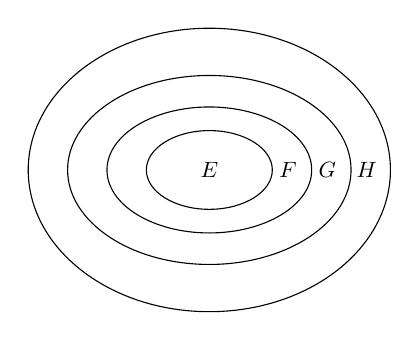
\begin{tikzpicture}[scale = 1,line join=round,line cap=round,>=stealth]
					\tikzset{every node/.style={scale=0.8}} 
					\draw (0,0) circle (0.8 and 0.5) circle (1.3 and 0.8) circle (1.8 and  1.2) circle (2.3 and 1.8);
					\path (0,0)  node {$E$}
						(1,0) node  {$F$}
						(1.5,0) node {$G$} 
						 (2,0) node {$H$};
				\end{tikzpicture}
		\end{center}
	} 
\end{ex}

% nguồn: MaHoaNH_TracNghiem_Lop10
\begin{ex}%[0D1H2-2]%[ma:beff4e08]
	Cho tập hợp $A=\left\{1;2;5;7\right\}$ và $B=\left\{1;2;3\right\}$. Có  tất cả bao nhiêu tập $X$ thỏa mãn $X\subset A$ và $X\subset B$?
	 \choice
		 {$2$}
		{\True $4$} 
		{$6$} 
		{$8$} 
	\loigiai{ 
		\begin{center}
			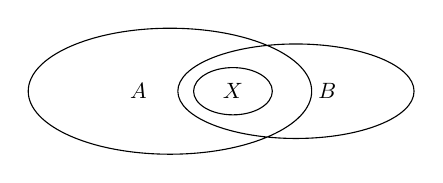
\begin{tikzpicture}[scale = 1,line join=round,line cap=round,>=stealth]
					\draw (0,0) circle (0.5 and 0.3) 
						 (-0.8,0) circle (1.8 and 0.8)
						(0.8,0) circle (1.5  and 0.6);
					\path (0,0) node {$X$} 
						(-1.2,0)  node {$A$}
						(1.2,0) node  {$B$};
				\end{tikzpicture}
		\end{center}
		Vì $\heva{&X\subset A\\&X\subset B}$ nên $X\subset \left(A\cap B\right)$. 
		Mà $A\cap B=\left\{1;2\right\}$  suy ra có $2^2=4$ tập $X$.
	} 
\end{ex}

% nguồn: MaHoaNH_TracNghiem_Lop10
\begin{ex}%[0D1H2-2]%[ma:21014b48]
	Cho hai tập hợp $A$ và $B$. Hình nào sau đây minh họa $A$ là tập con  của $B$?
	\begin{center}
		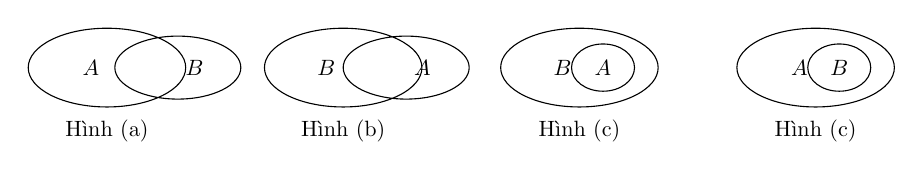
\begin{tikzpicture}[scale = 1,line join=round,line cap=round,>=stealth]
				 \tikzset{every node/.style={scale=0.8}}
				\draw (0,0) node[left]{$A$}circle (1 and 0.5)  node[yshift=-1.3cm,above]{Hình (a)}
					(0.9,0) node[right]{$B$}circle  (0.8 and 0.4);
				 \draw [shift={(3,0)}](0,0) node[left]{$B$}circle (1 and 0.5) node[yshift=-1.3cm,above]{Hình (b)}
					(0.8,0)  node[right]{$A$}circle (0.8 and 0.4);
				\draw [shift={(6,0)}](0,0) node[left]{$B$}circle (1 and 0.5) node[yshift=-1.3cm,above]{Hình (c)} 
					(0.3,0) node{$A$}circle  (0.4 and 0.3);
				\draw [shift={(9,0)}](0,0) node[left]{$A$}circle (1 and 0.5)  node[yshift=-1.3cm,above]{Hình (c)}
					(0.3,0) node{$B$}circle  (0.4 and 0.3);
			\end{tikzpicture}
	\end{center}
	 \choice
		{Hình (a)} 
		{Hình  (b)}
		 {\True Hình (c)}
		 {Hình (d)}
	\loigiai{Hình (c) là biểu đồ  ven, minh họa cho $A\subset B$ vì mọi phần tử của $A$ đều là của $B$.
	 }
\end{ex}

% nguồn: MaHoaNH_TracNghiem_Lop10
\begin{ex}%[0D1H2-2]%[ma:f304dce1]
	Khẳng định $A=B$ nào  sau đây {\bf sai}?
	\choice 
		 {$A=\{1;3\}, \; B=\left\{x\in \mathbb{R}\left|\left(x-1\right)\left(x-3\right)=0\right. \right\}$}
		{$A=\{1;3;5;7;9\},  B=\left\{n\in \mathbb{N}\left|n=2k+1, \; k\in \mathbb{Z},0\le k\le 4\right. \right\}$}
		{\True $A=\{-1;2\}, \;  B=\left\{x\in \mathbb{R}\left|x^2-2x-3=0\right. \right\}$}
		{$A=\varnothing, \; B=\left\{x\in  \mathbb{R}\left|x^2+x+1=0\right. \right\}$}
	 \loigiai{
		 Xét phương án $A=\{1;3\}, \; B=\left\{x\in \mathbb{R}\left|\left(x-1\right)\left(x-3\right)=0\right. \right\}$.
		\begin{itemize}
			\item $A=\{1;3\}$. 
			\item $B=\left\{x\in  \mathbb{R}\left|\left(x-1\right)\left(x-3\right)=0\right. \right\}\Rightarrow B=\left\{1; 3\right\}$.
		\end{itemize}
		Vậy $A=B$.\\ 
		Xét phương án $A=\{1;3;5;7;9\}, B=\left\{n\in \mathbb{N}\left|n=2k+1, \; k\in  \mathbb{Z},0\le k\le 4\right. \right\}$. Ta có
		\begin{itemize}
			\item  $A=\{1;3;5;7;9\}$.
			\item $B=\left\{n\in \mathbb{N}\left|n=2k+1, \; k\in \mathbb{Z},0\le k\le 4\right. \right\}\Rightarrow  B=\left\{1; 3; 5; 7; 9\right\}$.
		\end{itemize}
		 Vậy $A=B$.\\
		Xét phương án $A=\{-1;2\},  \; B=\left\{x\in \mathbb{R}\left|x^2-2x-3=0\right. \right\}$. Ta có
		\begin{itemize}
			 \item $A=\{-1;2\}$.
			\item $B=\left\{x\in  \mathbb{R}\left|x^2-2x-3=0\right. \right\}\Rightarrow B=\left\{-1; 3\right\}$.
		\end{itemize}
		Vậy $A\neq  B$.\\
		Xét phương án  $A=\varnothing, \; B=\left\{x\in \mathbb{R}\left|x^2+x+1=0\right. \right\}$. Ta có
		\begin{itemize}
			\item $A=\varnothing$. 
			\item $B=\left\{x\in  \mathbb{R}\left|x^2+x+1=0\right. \right\}\Rightarrow B=\varnothing$.
		\end{itemize}
		 Vậy $A=B$.
	 }
\end{ex}

% nguồn: MaHoaNH_TracNghiem_Lop10
\begin{ex}%[0D1K2-2]%[ma:f451df58]
	Có bao nhiêu tập hợp $X$ thoả mãn điều kiện $\left\{a, b\right\}\subset X \subset \left\{a, b, c, d, e\right\}$? 
	 \choice
		 {$2$}
		{$4$} 
		 {\True $8$}
		 {$10$}
	\loigiai{Từ điều kiện $\left\{a, b\right\}\subset X \subset \left\{a, b, c, d, e\right\}$ ta suy ra $X$ phải chứa các phần tử  $a, b$ và chỉ có thể thêm các phần tử $c, d, e$ nên chọn $X$ là một trong các tập hợp sau: $\left\{a, b \right\}$, $\left\{a, b, c \right\}$, $\left\{a, b, d \right\}$, $\left\{a, b, e \right\}$, $\left\{a, b, c, d \right\}$, $\left\{a, b, d, e \right\}$, $\left\{a, b, e, c \right\}$, $\left\{a, b, c, d, e \right\}$. Vậy có $8$ tâp hợp $X$ thoả mãn yêu cầu bài toán.}
\end{ex}

% nguồn: MaHoaNH_TracNghiem_Lop10
\begin{ex}%[0D1B2-2]%[ma:7d0d9794]
	Cho tập $A=\{0; 2; 4; 6\}$. Tập $A$ có bao nhiêu tập con có $2$  phần tử.
	 \choice
		{\True  $6$}
		{$4$} 
		 {$5$}
		{$1$} 
	\loigiai{Các tập con có $2$ phần tử là $\{0; 2\}$, $\{0; 4\}$, $\{0; 6\}$, $\{2; 4\}$, $\{2; 6\}$, $\{4; 6\}$.} 
\end{ex}

% nguồn: MaHoaNH_TracNghiem_Lop10
\begin{ex}%[0D1B2-2]%[ma:059a41cf]
	Số tập hợp con của tập hợp $A=\lbrace -3; 5  \rbrace$ là
	 \choice{$1$}
		 {$2$}
		{$3 $} 
		 {\True $4 $}
	\loigiai{Các  tập hợp $A=\lbrace -3; 5 \rbrace$ có $4$ tập hợp con là $\emptyset$, $\{-3\}$, $\{5\}$, $\{-3;5\}$.
	 }
\end{ex}

% nguồn: MaHoaNH_TracNghiem_Lop10
\begin{ex}%[0D1B2-2]%[ma:fff95e3e]
	 Cho tập hợp $K = \left\{x \in \mathbb{R} \mid 2x^2+x+18 = 0\right\}.$ Kết luận nào sau đây đúng?
	\choice{$K= \left\{0\right\} $} 
		{$K = 0 $} 
		{\True $K = \varnothing  $}
		{$K = \left\{\varnothing\right\}  $}
	 \loigiai{
	Ta có $ 2x^2+x+18 = 0$ vô nghiệm nên $K =  \varnothing $.}
\end{ex}

% nguồn: MaHoaNH_TracNghiem_Lop10
\begin{ex}%[0D1B2-2]%[ma:55e097d1]
	Trong các  mệnh đề sau, tìm mệnh đề \bf{sai}?
	\choice 
		 {\True $A \in A$}
		 {$\varnothing \subset A$}
		 {$A \subset A$}
		{$A \ne  \{A\}$}
	\loigiai{Ta  có $A \in A$ là mệnh đề sai.
	} 
\end{ex}

% nguồn: MaHoaNH_TracNghiem_Lop10
\begin{ex}%[0D1B2-2]%[ma:23013b2c]
	Cho tập hợp $A = [2;+\infty)$. Tập hợp $A$ {\bf không} là tập hợp con của tập hợp nào  sau đây?
	\choice 
		{ $M = \left\{x \in \mathbb{R} \mid  -2x+2 < 0 \right\} $ }
		{$N = \left\{x \in \mathbb{R} \mid -2x+4 \le  0 \right\} $}
		{\True $P = \left\{x \in \mathbb{R} \mid 3x-5 \le 0 \right\}  $}
		{  $Q = (-\infty;+\infty)$}
	\loigiai{ 
	Ta có $3x-5 \le 0 \Leftrightarrow x \le \dfrac{5}{3}.$} 
\end{ex}

% nguồn: MaHoaNH_TracNghiem_Lop10
\begin{ex}%[0D1K2-2]%[ma:695b5fb3]
	Cho tập hợp  $X = \left\{x \in \mathbb{R} \mid x > -1 \right\}$. Tập hợp nào trong các tập hợp sau đây {\bf không} chứa tập hợp $X$?
	\choice{\True $A =  [-3;7) $}
		 {$ \mathbb{R}$}
		{$ B  = [-3;+\infty)$}
		 {$ C = [-1; +\infty) $}
	 \loigiai{
		$X = \left\{x \in \mathbb{R} \mid x > -1 \right\}=(-1;+\infty)\not\subset A$  nên tập $A$ không chứa tập $X$.
	 }
\end{ex}

% nguồn: MaHoaNH_TracNghiem_Lop10
\begin{ex}%[0D1B2-2]%[ma:8b402ca3]
	Cho tập hợp $A=\{1;2;3\}$. Tập hợp nào sau đây \bf{không phải}  là tập con của tập $A$?
	 \choice
		{\True  $\{12;3\}$}
		 {$\varnothing$}
		{$A$} 
		 {$\{1;2;3\}$}
	\loigiai{Tập hợp không phải là  tập con của $A$ là $\{12;3\}$ vì $12 \notin A$.
	} 
\end{ex}

% nguồn: MaHoaNH_TracNghiem_Lop10
\begin{ex}%[0D1B2-2]%[ma:7aeaf2c4]
	Cho tập $X=\{2;3;4\}$. Hỏi tập hợp $X$ có bao nhiêu tập  hợp con?
	\choice 
		{  $7$}
		 {$6$}
		{$5$} 
		{\True $8$} 
	\loigiai{Số tập con của tập gồm $n$ phần tử là $2^n$. Tập $A$ có $3$ phần tử,  do đó có $2^3=8$ tập con.
	 }
\end{ex}

% nguồn: MaHoaNH_TracNghiem_Lop10
\begin{ex}%[0D1B2-2]%[ma:826a89e3]
	Cách viết nào sau đây \bf{không} đúng? 
	 \choice
		{\True $1 \subset  \mathbb{N}$}
		{$1  \in \mathbb{N}$}
		{$\{1\} \subset  \mathbb{N}$}
		{$1 \in \mathbb{N}^{\star}$} 
	\loigiai{Số $1$ là một phần tử  của tập số tự nhiên, do đó cách viết $1 \subset \mathbb{N}$ không đúng.
	} 
\end{ex}

% nguồn: MaHoaNH_TracNghiem_Lop10
\begin{ex}%[0D1B2-2]%[ma:c578c18b]
	Trong các  tập hợp sau, tập hợp nào bằng tập $\varnothing$?
	\choice{$ A= \left\{n \in \mathbb{N} \mid n^2  - 1 <0\right\}$}
		{$ B  = \left\{x \in \mathbb{R} \mid 2x+1= 0\right\}$}
		{$C= \left\{n \in  \mathbb{Z} \mid -2< n < 5 \right\} $}
		{\True $ D = \left\{x \in  \mathbb{R} \mid x^2+2x+2= 0\right\}$}
	\loigiai{ 
		Phương trình $x^2+2x+2=  0$ có $\Delta <0$ nên phương trình vô nghiệm hay $D=\varnothing$.
	 }
\end{ex}

% nguồn: MaHoaNH_TracNghiem_Lop10
\begin{ex}%[0D1B2-2]%[ma:e8123681]
	Số tập con của  tập $A=\{ 1;2;3\}$ là
	\choice 
		{\True  $8$}
		 {$6$}
		 {$5$}
		{$7$} 
	\loigiai{Số tập con của tập gồm  $n$ phần tử là $2^n$. Tập $A$ có $3$ phần tử, do đó có $2^3=8$ tập con.
	} 
\end{ex}

% nguồn: MaHoaNH_TracNghiem_Lop10
\begin{ex}%[0D1B2-2]%[ma:3ce5dfe7]
	Tính số các tập con có $2$ phần tử của  $M=\{1;2;3;4;5;6\}$.
	\choice 
		{\True  $15$}
		{$16$} 
		 {$18$}
		{$22$} 
	\loigiai{Số  tập con có $k$ phần tử của tập $X$ gồm $n$ phần tử là $\mathrm{C}_n^k$. Do đó số các tập con có $2$ phần tử của $M=\{1;2;3;4;5;6\}$ là $\mathrm{C}_6^2=15$.
	} 
\end{ex}

% nguồn: MaHoaNH_TracNghiem_Lop10
\begin{ex}%[0D1K2-2]%[ma:adb440c2]
	Cho hai đa thức $P(x)$ và $Q(x)$. Xét các tập hợp sau $A = \left\{x \in \mathbb{R}\big| P(x) = 0\right\}$ và \\ 
	$B = \left\{x \in \mathbb{R}\big| Q(x) = 0\right\}$, $C = \left\{x \in \mathbb{R}\big| P^2 (x) + Q^2 (x) = 0\right\}$. Khẳng định  nào sau đây \textbf{đúng}?
	 \choice{$A \subset C$}
		{$B \subset  C$}
		{\True $C \subset  A$}
		{$A  \subset B$}
	\loigiai{Ta có $P^2 (x) + Q^2 (x) = 0 \Leftrightarrow \heva{&P(x) = 0\\&Q(x) = 0}  \Rightarrow C$ gồm những phần tử để $P(x) = 0$ và $Q(x) = 0$ \\
	$\Rightarrow C  \subset A$.}
\end{ex}

% nguồn: MaHoaNH_TracNghiem_Lop10
\begin{ex}%[0D1B2-2]%[ma:d157202c]
	Cho tập hợp $X=\{0;1;2\}$. Tập $X$ có bao nhiêu  tập con?
	 \choice
		{\True $8$} 
		{$6$} 
		{$3$} 
		{$5$} 
	\loigiai{Tập $X$ có $3$ phần tử, do  đó nó có $2^3=8$ tập con.
	 }
\end{ex}

% nguồn: MaHoaNH_TracNghiem_Lop10
\begin{ex}%[0D1B2-2]%[ma:8873d571]
	Cho  tập hợp $A = [-2;1)$. $A$ là tập con của tập hợp nào sau đây?
	 \choice{$B=[-1;2)$}
		{\True $C = \left\{x \in \mathbb{R} \mid  -2 \le x < 1\right\} $}
		{$D= \left\{x \in \mathbb{Z} \mid -2 \le  x < 1\right\}$}
		 {$E= \left\{x \in \mathbb{N} \mid -2 \le x < 1\right\}$}
	\loigiai{ 
		$C = \left\{x \in  \mathbb{R} \mid -2 \le x < 1\right\} =[-2;1)$, suy ra $A\subset C$.
	 }
\end{ex}

% nguồn: MaHoaNH_TracNghiem_Lop10
\begin{ex}%[0D1B2-2]%[ma:84c9b50d]
	Cho $A=\{1;2;3\}$. Trong các khẳng định sau, khẳng định nào  \bf{sai}?
	 \choice
		 {$\varnothing \subset A$}
		{$1  \in A$}
		{$\{1;2\} \subset  A$}
		{\True $2=A$} 
	\loigiai{Ta có $2=A$ là khẳng định  sai.
	} 
\end{ex}

% nguồn: MaHoaNH_TracNghiem_Lop10
\begin{ex}%[0D1B2-2]%[ma:fcf353ae]
	Cho tập hợp $A = \left\{y \in  \mathbb{R} \mid y = x^2+x+1, \text{ với } x \in \mathbb{R}\right\}$. Tập hợp $A$ là tập hợp con của tập hợp nào sau đây?
	\choice{$M =  \left(-\infty;\dfrac{3}{4}\right] $}
		{$N = (3;+\infty)  $}
		{$P = \left(\dfrac{3}{4};+\infty\right)  $}
		{\True $U  = (0;+\infty) $}
	 \loigiai{
		 $y = x^2+x+1 = \left(x+\dfrac{1}{2}\right)^2+\dfrac{3}{4} \ge \dfrac{3}{4}$.
	} 
\end{ex}

% nguồn: MaHoaNH_TracNghiem_Lop10
\begin{ex}%[0D1B2-2]%[ma:81b4c1bf]
	Khẳng định nào  sau đây {\bf sai}?
	\choice{$ A \subset B \Leftrightarrow (\forall x, x \in A \Rightarrow x \in  B)$}
		{$(A \subset B) \text{  và } (B \subset C) \Rightarrow (A \subset C)$}
		{\True $\varnothing  $ không phải tập hợp con của $A$ với mọi tập hợp $A$}
		{$A=B \Leftrightarrow (A\subset B \text{ và } B  \subset A) $}
	 \loigiai{
		Tập rỗng là  tập con của mọi tập hợp.
	} 
\end{ex}

% nguồn: MaHoaNH_TracNghiem_Lop10
\begin{ex}%[0D1K2-2]%[ma:bf39d398]
	Tập hợp $A = \left\{1;2;3\right\}$ có bao nhiêu tập  con gồm hai phần tử?
	 \choice{$1$}
		{$2$} 
		 {\True $3$}
		{$4$} 
	 \loigiai{
		Số tập con của $ A $ gồm $ 2 $ phần tử là $ 3 $, đó là $ \left\{1;2\right\} $, $ \left\{2;3\right\}  $, $ \left\{1;3\right\} $.
	} 
\end{ex}

% nguồn: MaHoaNH_TracNghiem_Lop10
\begin{ex}%[0D1B2-2]%[ma:39edad6b]
	Cho tập hợp $A = \left\{y \in \mathbb{R} \mid y = 2x+1, \text{ với } x \in \mathbb{R} \text{ và } -2 \le  x < 3\right\}$. Tập $A$ bằng tập hợp nào sau đây?
	\choice{$M =  \left[-3;7\right] $}
		{ $N = [-2;3)$} 
		{\True $P =  \left\{x \in \mathbb{R} \mid -3 \le x < 7\right\}$}
		{$Q = \left\{y \in \mathbb{R} \mid -3 <  y \le 7 \right\}$}
	\loigiai{ 
		Ta  có $x = \dfrac{y-1}{2}$. Suy ra $ -2 \le \dfrac{y-1}{2} <3 \Leftrightarrow -3 \le y < 7$.
	} 
\end{ex}

% nguồn: MaHoaNH_TracNghiem_Lop10
\begin{ex}%[0D1K2-2]%[ma:32c2d64a]
	Cho  các tập hợp $A$ là tập hợp các tam giác, $B$ là tập hợp các tam giác đều, $C$ là tập hợp các tam giác cân. Khẳng định nào sau đây đúng?
	\choice{$A  = B$}
		{$A \subset B$} 
		 {$A \subset C$}
		{\True $B \subset  A$}
	 \loigiai{
		Tam giác đều là trường hợp đặc biệt của các  tam giác thường nên $B\subset A$.
	 }
\end{ex}

% nguồn: MaHoaNH_TracNghiem_Lop10
\begin{ex}%[0D1B2-2]%[ma:544b0f41]
	Trong các tập hợp sau,  tập hợp nào khác tập $\varnothing$?
	\choice{$ A= \left\{n \in \mathbb{N}  \mid n+1 = 0\right\}$}
		{ \True $ B = \left\{(x;y) \mid x,y \in \mathbb{R} \text{  và } x^2+y^2= 0\right\}$}
		{$C=  \left\{n \in \mathbb{Z} \mid n^2 = 2 \right\} $}
		{$ D = \left\{x \in \mathbb{R}  \mid -x^2+x-1= 0\right\}$}
	 \loigiai{
		Với $x=y=0$ ta có $x^2+y^2=0$ nên $B\ne \varnothing$. 
	} 
\end{ex}

% nguồn: MaHoaNH_TracNghiem_Lop10
\begin{ex}%[0D1Y2-2]%[ma:e4d3cd09]
	Cho tập hợp $A=\{a;b;c;d\}$. Số tập hợp con của $A$  có hai phần tử là
	 \choice
		 {$8$}
		 {$7$}
		 {\True $6$}
		 {$5$}
	 \loigiai{
	Các tập con có hai phần tử của tập $A$ là các tập $\{a;b\}$, $\{a;c\}$, $\{a;d\}$, $\{b;c\}$, $\{b;d\}$,  $\{c;d\}$. Suy ra có tất cả 6 tập.}
\end{ex}

% nguồn: MaHoaNH_TracNghiem_Lop10
\begin{ex}%[0D1B2-2]%[ma:0659d984]
	Cho ba tập hợp $M=\{n \in \mathbb{N} \mid n \; \vdots \; 5\}$, $P=\{n  \in \mathbb{N} \mid n \; \vdots \; 10\}$, $Q=\{x \in \mathbb{R} \mid x^2+3x+5=0\}$. Hãy chọn khẳng định đúng?
	\choice 
		{\True $Q  \subset P \subset M$}
		{$Q \subset M \subset P$} 
		{$M  \subset Q \subset P$}
		{$M  \subset P \subset Q$}
	 \loigiai{Ta có $M=\{5;10;15; \ldots \}$, $P=\{10,20,30, \ldots \}$, $Q=\varnothing$. Do đó $Q \subset P \subset M$.
	 }
\end{ex}

% nguồn: MaHoaNH_TracNghiem_Lop10
\begin{ex}%[0D1B2-2]%[ma:55982295]
	Cho tập $M=\{a;b;c;d;e\}$. Hãy chọn câu trả lời đúng  trong các câu sau
	\choice 
		{\True $M$ có  $32$ tập hợp con}
		{$M$ có $25$  tập hợp con}
		{$M$ có  $120$ tập hợp con}
		{$M$ có $5$  tập hợp con}
	\loigiai{Số tập  con của tập gồm $n$ phần tử là $2^n$. Tập $M$ có $5$ phần tử, do đó $M$ có $2^5=32$ tập con.
	 }
\end{ex}

% nguồn: MaHoaNH_TracNghiem_Lop10
\begin{ex}%[0D1B2-2]%[ma:e9b794bf]
	Cho $A=\{0;2;4;6\}$. Tập hợp $A$ có bao nhiêu tập hợp con có $3$ phần  tử?
	 \choice
		{\True  $4$}
		{$6$} 
		 {$7$}
		 {$8$}
	\loigiai{Các tập hợp con có $3$ phần tử là $\{0;2;4\}$, $\{0;2;6\}$, $\{0;4;6\}$,  $\{2;4;6\}$.\\
	 Có tất cả $4$ tập hợp con.}
\end{ex}

% nguồn: MaHoaNH_TracNghiem_Lop10
\begin{ex}%[0D1B2-2]%[ma:97737306]
	Cho tập hợp $A = \{n \in \mathbb{Z} \mid -2 < n \le 5\}$. Tập  hợp $A$ bằng tập hợp nào sau đây?
	\choice{$M = \{-1; 0;  1;2;3;4 \}$}
		 {$N = \{-1; 1;2;3;4; 5 \}$}
		 {\True $P = \{-1;0;1;2;3;4;5 \}$}
		{$Q = \{-2;-1; 0; 1;2;3;4 \}$} 
	 \loigiai{
		$A= \{n \in \mathbb{Z} \mid -2 < n \le 5\}=\{-1;0;1;2;3;4;5 \}=P$. 
	} 
\end{ex}

% nguồn: MaHoaNH_TracNghiem_Lop10
\begin{ex}%[0D1Y2-2]%[ma:ba055fb8]
	Cho tập hợp  $M=\{1;2;3;4;5\}$. Số các tập con của $M$ luôn chứa cả ba phần tử $1$, $3$, $5$ là
	 \choice
		 {$3$}
		 {$2$}
		{\True $4$} 
		{$8$} 
	 \loigiai{
		Các tập con của $M$ luôn chứa cả ba phần tử $1$, $3$, $5$ là  $\{1;3;5\}$, $\{1;3;5;2\}$, $\{1;3;5;4\}$, $\{1;3;5;2;4\}$.
	} 
\end{ex}

% nguồn: MaHoaNH_TracNghiem_Lop10
\begin{ex}%[0D1K2-2]%[ma:81ddb115]
	Cho hai đa thức $f\left(x\right)$ và $g\left(x\right)$ có cùng tập xác định và ba tập hợp $A = \left\{x \in \mathbb{R}\big| f\left(x\right) = 0\right\}$, $B = \left\{x \in \mathbb{R}\big| g\left(x\right) = 0\right\}$ và $C = \left\{x \in \mathbb{R}\big| f\left(x\right).g\left(x\right)  = 0\right\}$. Mệnh đề nào sau đây đúng?
	\choice{$A \subset  B$}
		{\True  $A \subset C$}
		{$C \subset A$} 
		 {$C \subset B$}
	 \loigiai{
		$f\left(x\right).g\left(x\right) =  0\Leftrightarrow \hoac{f(x)=0\\g(x)=0.}$\\
		Suy ra $A  \subset C$.
	 }
\end{ex}

% nguồn: MaHoaNH_TracNghiem_Lop10
\begin{ex}%[0D1B2-2]%[ma:7aa4c9b0]
	Tập hợp nào sau đây  có đúng một tập hợp con ?
	 \choice
		{$\left\{x,\varnothing\right\}$} 
		 {$\left\{x\right\}$}
		{$ \left\{\varnothing\right\}  $}
		{$ \True \varnothing $} 
	\loigiai{ 
	Tập  $ \varnothing $ có đúng một tập con là chính nó.
	} 
\end{ex}

% nguồn: MaHoaNH_TracNghiem_Lop10
\begin{ex}%[0D1B2-2]%[ma:710db092]
	Số tập hợp con của tập hợp  $ \{\varnothing\} $ là
	\choice 
		{$  1 $}
		{$ \True 2  $}
		{$ 3 $} 
		 {$ 4 $}
	 \loigiai{
	Tập $ \{\varnothing\} $ có hai tập con là $ \varnothing $ và  $ \{\varnothing\} $
	 }
\end{ex}

% nguồn: MaHoaNH_TracNghiem_Lop10
\begin{ex}%[0D1B2-2]%[ma:0fac3d50]
	Cho $A$ là tập hợp  các tam giác, $B$ là tập hợp các tam giác đều và $C$ là tập hợp các tam giác cân. Khẳng định nào sau đây là \textbf{đúng}?
	\choice 
		{$ A \subset B  \subset C $}
		{$ \True B \subset C  \subset A $}
		{$  C \subset B \subset A $}
		{$ A \subset C \subset  B $}
	\loigiai{ 
	Hiển  nhiên: $ B \subset C \subset A $
	} 
\end{ex}

% nguồn: MaHoaNH_TracNghiem_Lop10
\begin{ex}%[0D1B2-2]%[ma:76eaa441]
	Trong các mệnh  đề sau, mệnh đề nào \textbf{sai}?
	\choice 
		 {$\mathbb{N}\subset [0;+\infty)$}
		{$\left\{1;  3\right\}\subset [1; 3]$}
		{\True $[2; 5]=\left\{2; 3;  4; 5\right\}$}
		{$\varnothing \subset \mathbb{Q}$} 
	 \loigiai{
		Dễ thấy $ [2; 5]=\left\lbrace x\in\mathbb{R}\big |2\leq x\leq 5  \right\rbrace $ và $ \left\{2; 3; 4; 5\right\} $ là một tập hợp gồm $ 4 $ số tự nhiên nên $[2; 5]\neq \left\{2; 3; 4; 5\right\}$.
	 }
\end{ex}

% nguồn: MaHoaNH_TracNghiem_Lop10
\begin{ex}%[0D1B2-2]%[ma:8d504681]
	Cho các số thực $a$, $ b$, $ c$, $ d$ thoả  mãn $a<b<c<d$. Hãy chọn mệnh đề \textbf{sai} trong các mệnh đề sau.
	 \choice
		{\True $(a;c)\subset (c;d)$} 
		 {$(b;c)\subset (b;d)$}
		{$(b;c)\subset  (a;d)$}
		{$(a;c)\subset (a;d)$} 
	\loigiai{ 
		Dễ thấy $ (a;c)\cap  (c;d)=\varnothing$.
	} 
\end{ex}

% nguồn: MaHoaNH_TracNghiem_Lop10
\begin{ex}%[0D1B2-2]%[ma:ced123f0]
	Cho tập hợp $A=\left\{x\in \mathbb{R}\big||x-1|\leq 1 \right\}$.  $A$ bằng tập hợp nào trong các tập hợp sau?
	\choice 
		{$(0;1)$} 
		{$[0;1]$} 
		 {\True $[0; 2]$}
		 {$[-1;2]$}
	 \loigiai{
		Ta có $ |x-1|\leq 1\Leftrightarrow -1\leq x-1\leq 1\Leftrightarrow 0\leq x\leq  2 $.
	} 
\end{ex}

% nguồn: MaHoaNH_TracNghiem_Lop10
\begin{ex}%[0D1B2-2]%[ma:031dab69]
	Cho tập  hợp $A = \left\{x \in \mathbb{N}\big| x^2 + 8x + 15 = 0\right\}$. Khẳng định nào sau đây đúng?
	 \choice
		 {$A = \left\{-3;-5\right\}$}
		{\True $A  =\varnothing$}
		{$A  = \left\{\varnothing\right\}$}
		{$A  = \left\{0\right\}$}
	\loigiai{ 
		Phương trình $x^2+8x+15=0$ có hai nghiệm $x_1=-3$, $x_2=-5$. Tuy nhiên $x_1, x_2\notin  \mathbb{N}$. Vậy $A=\varnothing$.
	 }
\end{ex}

% nguồn: MaHoaNH_TracNghiem_Lop10
\begin{ex}%[0D1B2-2]%[ma:ab1d63a7]
	Tập hợp $A=\left\{x\in \mathbb{R}\big| 2>x>0 \right\}$ bằng tập  hợp nào dưới đây?
	 \choice
		{$(0;  2]$}
		{\True  $(0; 2)$}
		 {$[0; 2]$}
		{$\left\{0;  2\right\}$}
	\loigiai{ 
		$A=\left\{x\in \mathbb{R}\big| 2>x>0 \right\}=(0;2)$ theo  định nghĩa cá tập con của $\mathbb{R}$.
	 }
\end{ex}

% nguồn: MaHoaNH_TracNghiem_Lop10
\begin{ex}%[0D1B2-2]%[ma:ce28119b]
	Cho $A$  là tập hợp. Xác định mệnh đề đúng trong các mệnh đề sau đây
	\choice 
		{$\{\varnothing\}\subset  A$}
		{\True $\varnothing\subset A$} 
		{$A\cap\varnothing =A$} 
		{$A\cup\varnothing =\varnothing$} 
	 \loigiai{
		\lq\lq Với mọi tập $A$  bất kì, tập $\varnothing$ luôn là tập con của $A$.\rq\rq\
	} 
\end{ex}

% nguồn: MaHoaNH_TracNghiem_Lop10
\begin{ex}%[0D1B2-2]%[ma:741f6586]
	Cho tập hợp $A$  có $5$ phần tử. Hỏi tập hợp $A$ có bao nhiêu tập con.
	\choice 
		 {$16$}
		 {$10$}
		{$20$} 
		{\True $32$} 
	 \loigiai{
		Số tập con của tập $A$ là $2^5=32$. 
	 }
\end{ex}

% nguồn: MaHoaNH_TracNghiem_Lop10
\begin{ex}%[0D1K2-2]%[ma:6350147f]
	Cho H là tập hợp các hình  bình hành, V là tập hợp các hình vuông, T là tập hợp các hình thoi. Tìm mệnh đề sai
	\choice 
		 {$V \subset T$}
		{\True  $H \subset T$}
		{$T \subset  H$}
		{$V \subset  H$}
	\loigiai{ 
		 $H \subset T$
	} 
\end{ex}

% nguồn: MaHoaNH_TracNghiem_Lop10
\begin{ex}%[0D1B2-2]%[ma:d58f57d0]
	 Cho tập hợp $A=\{1;2;3;4\}$. Số tập hợp con gồm hai phần tử của tập hợp $A$ là
	 \choice
		 {$4$}
		{$8$} 
		 {$16$}
		 {\True $6$}
	 \loigiai{
		Các tập con gồm $2$ phần tử của tập $A$ là $\{1;2\}$; $\{1;3\}$; $\{1;4\}$;$\{2;3\}$; $\{2;4\}$; $\{3;4\}$. Vậy có $6$ tập con thỏa mãn yêu cầu  bài toán.
	} 
\end{ex}

% nguồn: MaHoaNH_TracNghiem_Lop10
\begin{ex}%[0D1B2-2]%[ma:bdf6ba09]
	Cho tập $A=\{a; b\}$, $B=\{a; b; c; d\}$. Có  bao nhiêu tập $X$ thỏa mãn $A\subset X\subset B$?
	 \choice
		{\True $4$} 
		 {$5$}
		 {$3$}
		{$6$} 
	 \loigiai{
		Các tập $X$ thỏa mãn là $\{a; b\}$,  $\{a; b; c\}$, $\{a; b; d\}$, $\{a; b; c; d\}$.
	 }
\end{ex}

% nguồn: MaHoaNH_TracNghiem_Lop10
\begin{ex}%[0D1B2-2]%[ma:4173a97a]
	Cho $A=\{1;2;3\}$, số tập con của  $A$ là
	\choice 
		 {$3$}
		{$5$} 
		 {\True $8$}
		{$6$} 
	 \loigiai{
		Số tập hợp con của tập  hợp $A$ là $2^3=8$.
	} 
\end{ex}

% nguồn: MaHoaNH_TracNghiem_Lop10
\begin{ex}%[0D1B2-2]%[ma:765e38f7]
	 Tập hợp nào sau đây có đúng một tập con?
	 \choice
		{$\{0\}$} 
		{$\{0;1\}$} 
		 {\True $\varnothing$}
		 {$\{1\}$}
	 \loigiai{
		Tập rỗng chỉ  có đúng một tập con là chính nó. Các tập có một phần tử trở lên luôn có ít nhất hai tập con là rỗng và chính nó.
	} 
\end{ex}

% nguồn: MaHoaNH_TracNghiem_Lop10
\begin{ex}%[0D1B2-2]%[ma:a0bc6f27]
	Cho tập hợp $X = \left\{x \in \mathbb{Z}\big| \left|2x + 1\right| \le 3\right\}$. Khẳng định  nào sau đây đúng?
	 \choice
		{$X = \left(-2;1\right)$} 
		{$X  = \left[-2;1\right]$}
		 {$X = \left\{-2;1\right\}$}
		{\True  $X = \left\{-2;-1;0;1\right\}$}
	\loigiai{ 
		Ta có $\left|2x + 1\right|  \le 3 \Leftrightarrow -3 \le 2x + 1 \le 3 \Leftrightarrow - 2 \le x \le 1 \Rightarrow X = \left\{-2;-1;0;1\right\}$.
	 }
\end{ex}

% nguồn: MaHoaNH_TracNghiem_Lop10
\begin{ex}%[0D1K2-2]%[ma:3714b9a7]
	Cho tập  hợp $A=\left\{1;2;3;a;b \right\}$. Số tập hợp con của $A$ là
	 \choice
		 {$5$}
		 {$8$}
		{\True$32$} 
		 {$10$}
	 \loigiai{
		Tập hợp $A$ có $5$ phần tử nên có $2^5=32$ tập hợp con. 
	 }
\end{ex}

% nguồn: MaHoaNH_TracNghiem_Lop10
\begin{ex}%[0D1B2-2]%[ma:2223d313]
	Cho tập hợp $A=\left\{x;y;z\right\}$ và  $B=\left\{x;y;z;t;u\right\}$. Có bao nhiêu tập $X$ thỏa mãn \break $A\subset X\subset B$?
	 \choice
		 {$16$}
		{\True  $4$}
		{$8$} 
		{$2$} 
	 \loigiai{
		Có $4$  tập hợp $X$ thỏa mãn $A\subset X\subset B$ là $X_1=\left\{{x;y;z}\right\}$; $X_2=\left\{{x;y;z;t}\right\}$; $X_3=\left\{{x;y;z;u}\right\}$ và $X_4=\left\{{x;y;z;t;u}\right\}$.
	} 
\end{ex}

% nguồn: MaHoaNH_TracNghiem_Lop10
\begin{ex}%[0D1B2-2]%[ma:bad90970]
	Ta gọi $H$ là tập hợp các hình bình hành, $V$ là tập hợp tất cả các hình vuông, $N$ là tập hợp tất cả các hình chữ nhật  và $T$ là tập hợp tất cả các hình tứ giác. Hãy tìm mệnh đề \textbf{sai} trong các mệnh đề sau.
	\choice 
		{$H\subset  T$}
		 {$V\subset N$}
		{$V\subset H$} 
		{\True  $N\subset V$}
	\loigiai{ 
		Ta có $ V\subset  N\subset H\subset T $.
	} 
\end{ex}

% nguồn: MaHoaNH_TracNghiem_Lop10
\begin{ex}%[0D1B2-2]%[ma:d903c639]
	Khẳng định  nào sau đây \textbf{sai} ?
	 \choice
		{$ \left\{-1,2\right\} \subset \mathbb{Z} $} 
		{$ \left\{1,\frac{2}{3}\right\} \subset \mathbb{Q}  $}
		{$ \True  \left\{1,\frac{2}{3}\right\} \subset \mathbb{Z} $}
		{$  \left\{1,\frac{2}{3}\right\} \subset \mathbb{R} $}
	\loigiai{ 
	Do $ \frac{2}{3} \notin \mathbb{Z} $  nên $ \left\{1,\frac{2}{3}\right\} \subset \mathbb{Z} $ là khẳng định sai.
	} 
\end{ex}

% nguồn: MaHoaNH_TracNghiem_Lop10
\begin{ex}%[0D1B2-2]%[ma:0585652b]
	Cho bốn tập hợp $ A,B,X,Y $ thỏa mãn: $ A \subset B $, $ B \subset X  $,$ X \subset Y $. Khẳng định nào sau đây \textbf{đúng} ?
	 \choice
		{$ X  \subset A $}
		{$ Y \subset B $} 
		{$ \True A  \subset Y $ }
		{$ A = B = X  $}
	 \loigiai{
	 Áp đụng tính chất tập hợp con, ta có: $ A \subset Y $.
	} 
\end{ex}

% nguồn: MaHoaNH_TracNghiem_Lop10
\begin{ex}%[0D1B2-2]%[ma:d8e3a3a1]
	Cho hai tập hợp $A = \left\{n \in \mathbb{Z}\big|  6\, \vdots\, n\right\}$ và $B = \left\{n \in \mathbb{Z}\big| 18\, \vdots\, n\right\}$. Khẳng định nào sau đây đúng?
	 \choice{$A = B$}
		{\True $A \subset  B$}
		{$B \subset  A$}
		{$A \in  B$}
	\loigiai{ 
		$A = \left\{n \in  \mathbb{Z}\big|6\,\vdots\, n\right\}=\{1;2;3\}$.\\
		$B  = \left\{n \in \mathbb{Z}\big| 18\, \vdots\, n\right\}=\{1;2;3;6;9;18\} $.\\
		Suy ra  $A \subset B.$
	} 
\end{ex}

% nguồn: MaHoaNH_TracNghiem_Lop10
\begin{ex}%[0D1K2-2]%[ma:3f94733c]
	Cho hàm số bậc nhất $ y=f(x) $ có $  f(-1)=2 $ và $ f(2)=-3 $. Hàm số đó là
	\choice 
		 {$y=-2x+3$}
		{$ y=\dfrac{-5x-1}{3}$} 
		{\True  $y=\dfrac{-5x+1}{3}$}
		 {$y=2x-3 $}
	\loigiai{ 
		Đặt $ y=f(x)=ax+b $. Ta có hệ phương trình $ \heva{&-a+b=2\\&2a+b=-3} \Leftrightarrow \heva{&a=-\dfrac{5}{3}\\&b=\dfrac{1}{3}} $.\\ 
		Vậy hàm số đó là $y=-\dfrac{5}{3}x+\dfrac{1}{3}$. 
	 }
\end{ex}

% nguồn: MaHoaNH_TracNghiem_Lop10
\begin{ex}%[0D1B2-2]%[ma:453f578e]
	Số tập con  có hai phần tử của tập $ A = \left\{1,2,3,4\right\} $ là
	 \choice
		 {$ 8 $}
		{$ \True  6 $}
		{$ 16  $}
		{$  7 $}
	\loigiai{ 
	Các tập con có hai phần tử của $  A $ là: $ \left\{1,2\right\},\left\{1,3\right\},\left\{1,4\right\},\left\{2,3\right\},\left\{2,4\right\},\left\{3,4\right\} $\\
	Vậy có  $ 6 $ tập thỏa mãn đề bài.
	} 
\end{ex}

% nguồn: MaHoaNH_TracNghiem_Lop10
\begin{ex}%[0D1B2-2]%[ma:cf49fcb2]
	Cho hai tập hợp $A=(2m-1;2m+3)$ và  $B=(-1;1)$ với tham số $m$. Có bao nhiêu giá trị nguyên của $m$ thỏa mãn $B\subset A$?
	 \choice
		{\True $2$} 
		 {$1$}
		{Vô  số}
		 {$0$}
	\loigiai{ 
	Ta có $B\subset A\Leftrightarrow  2m-1\le -1<1\le 2m+3\Leftrightarrow\heva{&m\le0\\&m\ge-1}\Leftrightarrow -1\le m\le0$.\\
	Chỉ có hai giá trị nguyên của $m$ thỏa mãn,  đó là $m=-1$ và $m=0$.
	} 
\end{ex}

% nguồn: MaHoaNH_TracNghiem_Lop10
\begin{ex}%[0D1K2-2]%[ma:23c21956]
	Cho tập $ A = \left\{n \in \mathbb{N}  \,|\, 1 \le n \le 5\right\}$ và tập $ \left\{B = n \in \mathbb{Z} \,|\, -2 \le n < 3\right\} $. Số các tập $ X $ thỏa mãn $ X \subset A $ và $ X \subset B $ là
	 \choice
		{$ 3  $}
		 {$ \True 4 $}
		{$ 2  $}
		{$ 5  $}
	 \loigiai{
	Ta có: $ A =\left\{{1,2,3,4,5}\right\} $ và $  B = \left\{-2,-1,0,1,2\right\} $\\
	Tập $ X $ thỏa mãn đề bài là một trong các tập sau $ \varnothing $,$  \left\{1\right\} $,$ \left\{2\right\} $,$ \left\{1,2\right\}$
	} 
\end{ex}

% nguồn: MaHoaNH_TracNghiem_Lop10
\begin{ex}%[0D1B2-2]%[ma:ef8d8725]
	Số các tập hợp  con của tập $ A = \left\{a,b,c\right\} $
	\choice 
		{$ \True  8 $}
		{$  5 $}
		{$  7 $}
		{$  6 $}
	 \loigiai{
	 Các tập hợp con của $ A $ là: $ \varnothing ,\left\{ a \right\},\left\{ b \right\},\left\{ c \right\},\left\{ a,b \right\},\left\{ a,c \right\},\left\{ b,c \right\},A $\\
	Vậy  tập $ A $ có $ 8 $ tập con.
	} 
\end{ex}

% nguồn: MaHoaNH_TracNghiem_Lop10
\begin{ex}%[0D1B2-2]%[ma:b4a3d83c]
	Cho tập hợp $T$ có $2$ phần  tử đôi một khác nhau. Số tập con của tập hợp $T$ là
	 \choice
		{$1$} 
		{$2$} 
		 {$3$}
		{\True  $4$}
	\loigiai{ 
		Giả  sử $ T=\{a,b\} $.
		Số tập con của tập hợp $  T $ là $ \varnothing $, $ \{a\} $, $ \{b\} $, $ \{a,b\} $. Vậy có $ 4 $ tập con.
	} 
\end{ex}

% nguồn: MaHoaNH_TracNghiem_Lop10
\begin{ex}%[0D1K2-2]%[ma:c9931846]
	 Cho hai tập hợp khác rỗng $A=\left[m-1;5\right)$ và $D=\left[-3;2m+1\right]$. Tìm $m$ để $A\subset D$.
	\choice 
		{\True  $2 \le m <6$}
		{$-2 \le m  <6$}
		 {$m\le 2$}
		 {$m\le-2$}
	\loigiai{ 
		Điều kiện $\heva{& m-1 < 5 \\ & -3<2m+1} \Leftrightarrow \heva{& m < 6 \\ & m>-2}\Leftrightarrow -2< m < 6$.\\ 
		Để $A\subset D$ thì $\heva{& m-1\geqslant-3 \\ & 5\leqslant 2m+1}\Leftrightarrow \heva{&  m\geqslant -2\\ & m\geqslant 2}\Leftrightarrow 2\leqslant m<6$.\\
	Kết hợp với điều kiện suy ra $2\leqslant  m<6$.}
\end{ex}

% nguồn: MaHoaNH_TracNghiem_Lop10
\begin{ex}%[0D1B2-2]%[ma:468b4c41]
	Cho tập hợp $ A = \left\{a,b,c,d,e\right\} $. Số các tập con của tập $  A $ có ba phần tử và luôn chứa phần tử $ a $ là
	\choice 
		 {\True 6}
		{$  5 $}
		{$ 7  $}
		 {$ 8 $}
	 \loigiai{
	Các tập con của $ A $  thỏa mãn đề bài là: $ \left\{a,b,c\right\},\left\{a,b,d\right\},\left\{a,b,e\right\},\left\{a,c,d\right\},\left\{a,c,e\right\},\left\{a,d,e\right\} $\\
	 Vậy có $ 6 $ tập thỏa mãn đề bài.
	} 
\end{ex}

% nguồn: MaHoaNH_TracNghiem_Lop10
\begin{ex}%[0D1K2-2]%[ma:7a2fc750]
	Cho tập hợp $P=\{1,2,3,4,5,6\}$, số các tập con của $P$ chứa  cả ba phần tử $3$, $4$, $5$ là
	\choice 
		{$3$} 
		 {$5$}
		 {$6$}
		 {\True $8$}
	 \loigiai{
		Ta thấy $P=\{3,4,5\}\cup \{1,2,6\}$  suy ra số tập con của $P$ chứa cả ba phần tử $3$, $4$, $5$ cũng bằng số tập con của tập hợp $\{1,2,6\}$. Bằng cách liệt kê các tập con ta thấy tập hợp $\{1,2,6\}$ có tất cả $8$ tập con.\\
		Vậy có $8$ tập hợp theo yêu  cầu bài toán.
	 }
\end{ex}

% nguồn: MaHoaNH_TracNghiem_Lop10
\begin{ex}%[0D1B2-2]%[ma:720254a8]
	Biết rằng $ A $ là tập hợp các hình tứ giác,  $ B $ là tập hợp các hình bình hành, $ C $ là tập hợp các hình chữ nhật, $ D $ là tập hợp các hình thoi và $ E $ là tập hợp các hình vuông. Khẳng định nào sau đây \textbf{sai} ?
	\choice 
		 {$ E \subset C \subset B \subset A $}
		{$ E \subset  D \subset B \subset A $}
		{$ E \subset C \subset  A $}
		{$ \True E  \subset D \subset C \subset B $}
	 \loigiai{
	Mọi hình vuông đều có thể coi là hình thoi, nhưng mọi hình thoi không thể coi là hình  chữ nhật nên $ E \subset D \not\subset C $.\\
	 Vậy $ E \subset D \subset C \subset B $ là khẳng định sai.
	 }
\end{ex}

% nguồn: MaHoaNH_TracNghiem_Lop10
\begin{ex}%[0D1B2-2]%[ma:e0513b8b]
	Cho tập $A=\{x \in \mathbb{N}\mid (2-x)(x^2-5x-6)=0\}$. Hỏi tập  $A$ có bao nhiêu tập con?
	 \choice
		 {$2$}
		 {\True $4$}
		{$3$} 
		 {$8$}
	\loigiai{ 
		Ta có $(2-x)(x^2-5x-6)=0 \Leftrightarrow  \hoac{&x=2 \in \mathbb{N}\\& x=-1 \notin \mathbb{N}\\& x=6 \in \mathbb{N}.}$\\
		Suy  ra $A=\{2;6\}$.\\
	Do đó $A$ có các tập con  là: $\{2\};\{4\};\{2;6\};\varnothing$.}
\end{ex}

% nguồn: MaHoaNH_TracNghiem_Lop10
\begin{ex}%[0D1B2-2]%[ma:921cc1e8]
	Cho hai tập hợp $ X = \left\{n \in \mathbb{N} \,|\, n \text{ là bội số của } 4 \text{ và } 6\right\}  $, $ Y = \left\{n \in \mathbb{N} \,|\, n \text{ là bội số của } 12 \right\} $. Trong các mệnh đề sau, mệnh đề nào \textbf{sai} ?
	 \choice
		{$ X \subset Y  $}
		{$ Y \subset X $} 
		 {$ X = Y $}
		{$ \True \exists n  \in \mathbb{N} \,:\, n \in X \text{ và } n \notin Y $}
	 \loigiai{
	Ta có: $ X = \left\{0,12,24,36,\ldots\right\} $  và $ Y = \left\{0,12,24,36,\ldots\right\} $ nên $ X = Y $ là khẳng định đúng.\\
	Suy ra $  X \subset Y $ , $ Y \subset X $ cũng là khẳng định đúng.
	 }
\end{ex}

% nguồn: MaHoaNH_TracNghiem_Lop10
\begin{ex}%[0D1B2-2]%[ma:345b957b]
	Cho hai tập hợp $ A = \left\{ 3k+1\,|\,k \in \mathbb{Z} \right\}$ và  $ B = \left\{6l+4\,|\,l \in \mathbb{Z} \right\} $. Khẳng định nào sau đây \textbf{đúng} ?
	\choice 
		 {$ B \not\subset A $}
		{$ A = B  $}
		{$ A \subset B $} 
		{$ \True  B \subset A $}
	\loigiai{ 
	Giả sử $ x $ là một phần tử tùy ý của $ B $, khi đó $ x = 6l+4 = 3(2l+1) = 3k+1 $, với  $ k = 2l+1 \Rightarrow x \in A $\\
	Vậy $ \forall x  \in B \Rightarrow x \in A$ hay $ B \subset A $.
	 }
\end{ex}

% nguồn: MaHoaNH_TracNghiem_Lop10
\begin{ex}%[0D1B2-2]%[ma:f79e8e84]
	Cho biết $x$ là một phần tử  của tập hợp $A$. Xét các mệnh đề sau
	\[(I): x \in A; \; (II): \{x\} \in A;  \; (III): x \subset A; \; (IV): \{x\} \subset A \]
	Hỏi trong các mệnh đề trên, mệnh  đề nào đúng?
	 \choice
		{\True  $(I)$ và $(IV)$}
		 {$(I)$ và $(III)$}
		{$(I)$  và $(II)$}
		{$(II)$ và $(IV)$} 
	\loigiai{Cho $x$ là một phần tử của tập hợp $A$. Khi đó  $x \in A$ và $\{x\} \subset A$.
	} 
\end{ex}

% nguồn: MaHoaNH_TracNghiem_Lop10
\begin{ex}%[0D1Y2-2]%[ma:ff436e59]
	Cho tập $A=\{a;b;5\}$. Số tập con  của tập $A$ là
	 \choice
		{$5$} 
		{$4$} 
		 {$7$}
		{\True  $8$}
	\loigiai{ 
		Tập con của $A$ là $\varnothing, \{a\}, \{b\},\{5\}, \{a;b\}, \{a;5\}, \{b;5\}, \{a;b;5\} $.  Vậy số tập con của $A$ là $8$.\\
		Có thể dùng  công thức $2^3=8$ tập con.
	} 
\end{ex}

% nguồn: MaHoaNH_TracNghiem_Lop10
\begin{ex}%[0D1K2-2]%[ma:5bae9623]
	Cho hai tập khác rỗng $ A=[m-3;  1), B=(-3; 4m+5) $ với $ m\in\mathbb{R} $. Tìm tất cả các giá trị của tham số $ m $ để tập $ A $ là tập con của tập $ B $.
	 \choice
		{$ m\geq  0 $}
		{\True $ 0<m<4 $} 
		{$  m\geq -1 $}
		 {$ m>0 $}
	 \loigiai{
		Vì $ A, B $ khác rỗng và $ A\subset B $ nên $$\heva{& m-3<1\\ & -3<4m+5\\ & -3< m-3\\  & 1\leq 4m+5}\Leftrightarrow\heva{& m<4\\ & m>-2\\ & m>0\\ &m\geq -1}\Leftrightarrow 0<m<4.$$
		Vậy giá trị  $ m $ cần tìm là $ 0<m<4$.
	} 
\end{ex}

% nguồn: MaHoaNH_TracNghiem_Lop10
\begin{ex}%[0D1B2-2]%[ma:4c11a56a]
	Có bao nhiêu tập hợp $X$ thỏa mãn $\left\{{a,b}\right\}\subset X\subset\left\{{a, b, c, d,  e}\right\}$?
	 \choice
		 {$5$}
		 {$6$}
		 {$7$}
		 {\True $8$}
	\loigiai{ 
		Vì $\left\{{a,b}\right\}\subset X$ nên tập $X$ có ít nhất hai phần tử  $a$ và $b$.\\
		Mặt khác $X\subset\left\{{a, b, c,  d, e}\right\}$ nên tập $X$ có tối đa năm phần tử và $c, d, e \in X$.\\
		Vậy tất cả các tập $X$ thỏa mãn là $\{a, b\}$; $\{a, b, c\}$; $\{a, b, d\}$; $\{a, b, e\}$; $\{a, b, c, d\}$; $\{a, b, d, e\}$; $\{a, b, c, e\}$; $\{a, b, c, d,  e\}$.
	} 
\end{ex}

% nguồn: MaHoaNH_TracNghiem_Lop10
\begin{ex}%[0D1K2-2]%[ma:d82bf58a]
	Cho tập $X$ có $n+1$ phần tử ($n\in \mathbb{N}$). Số tập con của $X$ có hai  phần tử là
	\choice 
		{$n(n+1)$} 
		{$\dfrac{n(n-1)}{2}$} 
		{$n+1$} 
		{\True  $\dfrac{n(n+1)}{2}$}
	 \loigiai{
		Lấy một phần tử của $X$, ghép với $n$ phần tử còn lại được $n$  tập con có hai phần tử.\\
		Vậy có $(n+1)n$  tập.\\
		Nhưng mỗi tập con đó được tính hai  lần nên số tập con của $X$ có hai phần tử là $\dfrac{n(n+1)}{2}$.
	} 
\end{ex}

% nguồn: MaHoaNH_TracNghiem_Lop10
\begin{ex}%[0D1B2-2]%[ma:ff80672c]
	Tập hợp nào sau đây có đúng một tập hợp  con?
	\choice 
		{\True $\varnothing  $}
		{$\left\lbrace 1 \right\rbrace  $}
		 {$\left\{\varnothing \right\}$}
		{$\left\{1;\varnothing  \right\}$}
	\loigiai{ 
		Tập $\varnothing $ duy nhất một tập con là  $\varnothing $.\\
		 Tập $\left\lbrace 1 \right\rbrace $ còn một tập con nữa là tập $\varnothing $.\\
		Tập $\left\{\varnothing \right\}$ có hai tập con là $\varnothing $  và $\left\{\varnothing \right\}$.\\
	Tập $\left\{1;\varnothing \right\}$ có ba tập con $\left\{\varnothing \right\}$,  $\{1\}$ và $\left\{1;\varnothing \right\}$.}
\end{ex}

% nguồn: MaHoaNH_TracNghiem_Lop10
\begin{ex}%[0D1B2-2]%[ma:02abcfe6]
	Cho các tập $ A = \left\{x \in \mathbb{R} \,|\, x^2-3x+2=0\right\} $, $ B = \left\{a,2\right\} $, $ C = \left\{1,b\right\} $. Biết $ A = B = C $, khi đó tổng $ T = a  + b $ là
	 \choice
		{$ T =  2 $}
		{$ T = 7  $}
		{$  \True T = 3 $}
		{$ T =  5 $}
	\loigiai{ 
	Phương trình $ x^2-3x+2 = 0 $ có hai nghiệm  là $ 1 $ và $ 2 $ nên tập $ A = \left\{1,2\right\} $\\
	Do $ B = A $ nên $ a = 1 $, $ C = A $ nên $  b = 2 $\\
	Vậy $ T = 1 + 2 = 3  $.
	} 
\end{ex}

% nguồn: MaHoaNH_TracNghiem_Lop10
\begin{ex}%[0D1B2-2]%[ma:ac71565e]
	Tập hợp nào  sau đây có đúng hai tập hợp con?
	 \choice
		 {$\left\{x;\varnothing \right\}$}
		{\True $\{x\}$} 
		{$\left\{x;y;\varnothing  \right\}$}
		{$\{x;y\}$} 
	\loigiai{ 
		\begin{itemize}
			\item Công  thức số tập con của tập hợp có $n$ phần tử là $2^n$ nên suy ra tập $\{x\}$ có 1 phần tử nên có $2^1=2$ tập con.
			\item Liệt  kê số tập con ra thì $\{x\}$ có hai tập con là $\{x\}$ và $\left\{\varnothing \right\}$.
		\end{itemize}
	} 
\end{ex}

% nguồn: MaHoaNH_TracNghiem_Lop10
\begin{ex}%[0D1K2-2]%[ma:178472ff]
	Cho tập hợp $ A = \left\{1,2,3\right\} $ và  $ B = \left\{1,2,3,4,5\right\} $. Số các tập $ X $ thỏa mãn $ A \subset X \subset B $
	 \choice
		 {$ 1 $}
		{$ 3 $} 
		 {$ 2 $}
		{$ \True 4  $}
	 \loigiai{
	$  A \subset X \Rightarrow 1,2,3 \in X $\\
	$ X \subset B \Rightarrow X $ có thể có thêm các phần tử  $ 4,5 $\\
	Khi đó, tập $ X $ là một  trong các tập sau: $ \left\{1,2,3\right\} $,$ \left\{1,2,3,4\right\} $,$ \left\{1,2,3,5\right\} $,$ \left\{1,2,3,4,5\right\} $\\
	Vậy có $ 4 $ tập  $ X $ thỏa mãn đề bài.
	} 
\end{ex}

% nguồn: MaHoaNH_TracNghiem_Lop10
\begin{ex}%[0D1K2-2]%[ma:aa061884]
	Cho tập hợp $A=\{0;1;2;3;4;5;6;7;8;9\}$. Số  tập hợp con có đúng $ 2 $ phần tử của $A$ là
	\choice 
		 {$5$}
		{$9$} 
		 {\True $45$}
		 {$90$}
	\loigiai{ 
		\textbf{Cách 1:  }
		Số tập con của tập $A$ gồm  $ 2 $ phần tử là số cách lấy ra bộ $ 2 $ số từ $A$.\\
		Do đó có số tập con là $\dfrac{10\cdot 9}{2}=45$ (Bộ hai số  lấy ra $a,b$ trùng với $b,a$).\\
		\textbf{Cách 2: } Số tập hợp con có đúng $ 2 $ phần tử của $A$ bằng số các số tự  nhiên có hai chữ số $\overline{ab}$, với $a>b$ $(*)$.\\
		Số các số tự nhiên có hai chữ số là $100-10=90$ số. Trong đó, có $9$ số $10; 20; \ldots; 90$ thỏa mãn $(*)$; có $9$  số $11; 22; \ldots; 99$ không thỏa mãn $(*)$; và số các số còn lại thỏa mãn $(*)$ là $\dfrac{90-9-9}{2}=36$. Vậy tổng số các số thỏa mãn $(*)$ là $9+36=45$.
	 }
\end{ex}

% nguồn: MaHoaNH_TracNghiem_Lop10
\begin{ex}%[0D1K2-2]%[ma:7f45660b]
	Cho tập hợp $A=\left\lbrace 1;2;3;a;b;c\right\rbrace $. Số tập con có $3$  phần tử của tập $A$ trong đó có ít nhất một chữ số là
	\choice 
		{$21$} 
		{$18$} 
		 {$20$}
		{\True  $19$}
	 \loigiai{
		\begin{itemize}
			\item Trường hợp  có $3$ chữ số, có $1$ tập: $\left\lbrace 1;2;3\right\rbrace $.
			\item Trường hợp có $2$ chữ số, có $9$ tập: $\left\lbrace 1;2;a\right\rbrace $, $\left\lbrace 1;2;b\right\rbrace $, $\left\lbrace 1;2;c\right\rbrace $,  $\left\lbrace 1;3;a\right\rbrace $, $\left\lbrace 1;3;b\right\rbrace $, $\left\lbrace 1;3;c\right\rbrace $, $\left\lbrace 2;3;a\right\rbrace $, $\left\lbrace 2;3;b\right\rbrace $, $\left\lbrace 2;3;c\right\rbrace $.
			\item Trường hợp có $1$ chữ số, có $9$ tập: $\left\lbrace 1;a;b\right\rbrace $, $\left\lbrace 1;a;c\right\rbrace $, $\left\lbrace  1;b;c\right\rbrace $, $\left\lbrace 2;a;b\right\rbrace $, $\left\lbrace 2;a;c\right\rbrace $, $\left\lbrace 2;b;c\right\rbrace $, $\left\lbrace 3;a;b\right\rbrace $, $\left\lbrace 3;a;c\right\rbrace $, $\left\lbrace 3;b;c\right\rbrace $.
		\end{itemize}
		Vậy có tất cả  $19$ tập thỏa đề bài.
	} 
\end{ex}

% nguồn: MaHoaNH_TracNghiem_Lop10
\begin{ex}%[0D1K2-2]%[ma:89ca26f8]
	Tập  hợp $Y = \left\{2;3;4\right\}$ có bao nhiêu tập hợp con?
	\choice{$\True  8$}
		{$5$} 
		 {$3$}
		{$1$} 
	\loigiai{ 
		\begin{itemize}
			\item Số tập con của  $ Y $ gồm $ 0 $ phần tử là $ 1 $.
			\item Số tập con của $ Y $ gồm $ 1 $ phần tử là  $ 3 $.
			\item Số tập con của $ Y $ gồm $  2 $ phần tử là $ 3 $.
			\item Số tập con của $ Y $ gồm $ 3 $ phần tử  là $ 1 $.
		\end{itemize}
		Vậy có tất cả  $ 8 $ tập con của $ Y $.
	 }
\end{ex}

% nguồn: MaHoaNH_TracNghiem_Lop10
\begin{ex}%[0D1K2-2]%[ma:e3316a8b]
	Cho hai tập hợp  $A=[1;3]$ và $B=[m;m+1]$. Tìm tất cả giá trị của tham số $m$ để $B\subset A$.
	 \choice
		 {$m=1$}
		{$1<m<2$} 
		{\True $1\leqslant m\leqslant 2$} 
		{$m=2$} 
	\loigiai{ 
		Ta có: $B\subset A \Leftrightarrow \left\{\begin{aligned}
		&m\geqslant 1\\ 
		&m+1\leqslant 3\\ 
	\end{aligned}\right. \Leftrightarrow \left\{\begin{aligned}
	&m\geqslant 1\\ 
	&m\leqslant  2\\
	\end{aligned}\right. $. Vậy $1\leqslant m\leqslant 2$.}
\end{ex}

% nguồn: MaHoaNH_TracNghiem_Lop10
\begin{ex}%[0D1K2-2]%[ma:3faf1bc0]
	Cho các  tập hợp $A=\left[m+1;7\right)$, $D=\left[-4;2m+1\right]$. Có bao nhiêu giá trị nguyên của $m$ để $A\subset D$?
	 \choice
		{$  2$}
		 {\True $ 3 $}
		 {$ 4 $}
		{$5 $} 
	\loigiai{ 
		Điều kiện 
		 $\heva{&m+1 <7 \\ &2m+1>-4 }
		\Leftrightarrow 
		\heva{&m<6 \\ &m>-\dfrac{5}{2} } 
		\Leftrightarrow  -\dfrac{5}{2}<m<6.\\$
		Ta có $A\subset D  \Leftrightarrow
		 \heva{& m+1 \ge -4 \\ &2m+1\ge 7 }
		\Leftrightarrow 
		 \heva{&m \ge -5 \\ &m\ge 3 }
		 \Leftrightarrow m\ge 3.\\$
		Kết hợp với điều kiện suy ra $ 3\leq  m <6 $.\\
		Vì $m \in \mathbb{Z}$ nên $m \in \left\{{3; 4; 5}\right\}$. 
	} 
\end{ex}

% nguồn: MaHoaNH_TracNghiem_Lop10
\begin{ex}%[0D1B2-2]%[ma:6ce297c7]
	Cho các tập hợp $A = \left(-1;3\right)$, $B = \left(-\infty;4\right)$ và  $C = \left[-1;3\right]$. Khẳng định nào sau đây đúng?
	\choice{$B \subset  A$}
		{$B \subset C$} 
		{\True  $C \subset B$}
		{$C  \subset A$}
	\loigiai{ 
	\immini{ 
		Dựa vào trục số biểu diễn các  tập hợp $ A $, $ B $, $ C $ ta dễ thấy $C \subset B$.
		 }{
		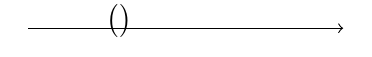
\begin{tikzpicture}
				 \draw[->](-1,0)->(3,0);
				 \IntervalLR{-0.9}{-0.5}
				\def\skipInterval{0.5cm} 
				\IntervalGR{}{}{\big  (}{-2}
				\IntervalLR{1}{2.8} 
				 \def\skipInterval{0.5cm}
				 \IntervalGR{\big)}{0}{}{}
			\end{tikzpicture}
		\\ 
		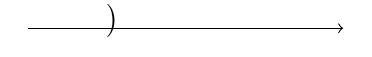
\begin{tikzpicture}
				\draw[->](-1,0)->(3,0); 
				 \IntervalLR{2.5}{2.8}
				 \def\skipInterval{0.5cm}
				\IntervalGR{\big)}{4}{}{} 
			\end{tikzpicture}
		 \\
		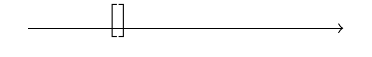
\begin{tikzpicture}
				 \draw[->](-1,0)->(3,0);
				\IntervalLR{-0.9}{0} 
				\def\skipInterval{0.5cm} 
				\IntervalGR{}{}{\big [}{-1} 
				 \IntervalLR{2}{2.8}
				\def\skipInterval{0.5cm} 
				 \IntervalGR{\big]}{2}{}{}
			\end{tikzpicture}
		 }
	} 
\end{ex}


%%%%%%%%%%%%%%%% ĐÚNG/SAI %%%%%%%%%%%%%%%%

% nguồn: MaHoaNH_DungSai_Lop10
\begin{ex}%[0D1N2-2]%[ma:73607365]
	Các câu sau  là đúng hay sai?
	 \choiceTF
		{$\left\{x\in\mathbb{R}\Big|-2<x<3\right\}=[-2;3]$} 
		{$\left\{x\in\mathbb{R}\Big|1\leq slant  x\leq slant10\right\}=(1;10)$}
		 {\True $\left\{x\in\mathbb{R}\Big|-5<x\leq slant\sqrt{3}\right\}=\left(-5;\sqrt{3}\right]$}
		{\True  $\left\{x\in\mathbb{R}\Big|\pi\leq slant x<4\right\}=[\pi;4)$}
	\loigiai{ 
	\begin{itemchoice}
		 \itemch $\left\{x\in\mathbb{R}\Big|-2<x<3\right\}=(-2;3)$.
		\itemch $\left\{x\in\mathbb{R}\Big|1\leq slant x\leq slant10\right\}=[1;10]$. 
		\itemch  $\left\{x\in\mathbb{R}\Big|-5<x\leq slant\sqrt{3}\right\}=\left(-5;\sqrt{3}\right]$.
		 \itemch $\left\{x\in\mathbb{R}\Big|\pi\leq slant x<4\right\}=[\pi;4)$.
	\end{itemchoice}
	 }
\end{ex}

% nguồn: MaHoaNH_DungSai_Lop10
\begin{ex}%[0D1N2-2]%[ma:74bd1697]
	Các  câu sau là đúng hay sai?
	\choiceTF 
		{\True Với hai tập $A=\left\{-\sqrt{3};\sqrt{3}\right\}$ và  $B=\left\{x\in\mathbb{R}\Big|x^2-3=0\right\}$, ta có $A=B$}
		{\True Với $C$ là tập  hợp các tam giác đều và $D$ là tập hợp các tam giác cân, ta có $C\subset D$}
		{Với hai tập $E=\left\{x\in\mathbb{N}\Big|x \text{ là ước của  } 12\right\}$ và $F=\left\{x\in\mathbb{R}\Big|x \text{ là bội của } 24\right\}$, ta có $F\subset E$}
		{Tất cả các tập con của  tập $\{g;h\}$ là $\{g\}$, $\{h\}$, $\{g;h\}$}
	 \loigiai{
	\begin{itemchoice}
		\itemch Ta có $x^2-3=0 \Leftrightarrow \hoac{ &  x=-\sqrt{3} \\ & x=\sqrt{3}} \Rightarrow B=\left\{-\sqrt{3};\sqrt{3}\right\}$. \\
		 Vậy $A=B$.
		\itemch Vì tam giác đều là  tam giác cân nên $C\subset D$.
		\itemch Với $x=24$, ta có $x\in F$  nhưng $x\notin E$ nên $F\not\subset E$.
		\itemch Tất cả các tập con của tập $\{g;h\}$ là $\varnothing$, $\{g\}$, $\{h\}$,  $\{g;h\}$.
	\end{itemchoice}
	 }
\end{ex}

% nguồn: MaHoaNH_DungSai_Lop10
\begin{ex}%[0D1N2-2]%[ma:1ec78a00]
	Các câu sau là  đúng hay sai?
	 \choiceTF
		{Với hai tập  $A=\{0;1;2;3;4\}$ và $B=\{0;2;4\}$, ta có $A\subset B$}
		{\True Với hai tập $C=\left\{x\in\mathbb{R}\Big|x^2=4\right\}$ và $D=\left\{x\in\mathbb{R}\Big||x|=2\right\}$, ta có $C=D$} 
		{\True Với $E$  là tập các hình bình hành và $F$ là tập các tứ giác có hai cặp cạnh đối song song, ta có $E=F$}
		{Với hai tập $G=\left\{x\in\mathbb{N}\Big|x \text{ là bội của } 3\right\}$ và $H=\left\{x\in\mathbb{N}\Big|x \text{ là bội của } 6\right\}$, ta có  $G\subset H$}
	\loigiai{ 
	\begin{itemchoice}
		\itemch  Ta có $1\in A$ nhưng $1\notin B$ nên $A\not\subset B$.
		\itemch Ta có $x^2=4 \Leftrightarrow \hoac{ & x=-2 \\ & x=2} \Rightarrow C=\{-2;2\}$. \\ 
		Ta có $|x|=2 \Leftrightarrow  \hoac{ & x=-2 \\ & x=2} \Rightarrow D=\{-2;2\}$. \\
		Vậy  $C=D$.
		\itemch Ta  có $E=F$.
		\itemch Với  $x=3$, ta có $x\in G$ nhưng $x\notin H$ nên $G\not\subset H$.
	\end{itemchoice}
	 }
\end{ex}

% nguồn: MaHoaNH_DungSai_Lop10
\begin{ex}%[0D1H2-2]%[ma:ecb0dcb0]
	Các câu sau là  đúng hay sai?
	 \choiceTF
		 {\True $(-2\pi;2\pi]\subset(-\infty;10)$}
		{$(-1;1)\setminus(-\infty;2]=(-1;1)$} 
		{$(-\infty;3)\cap(-3;+\infty)=\varnothing$} 
		 {$(-\infty;-2)\cup(2;+\infty)=\mathbb{R}$}
	 \loigiai{
	\begin{itemchoice}
		 \itemch $(-2\pi;2\pi]\subset(-\infty;10)$.
		\itemch  $(-1;1)\setminus(-\infty;2]=\varnothing$.
		\itemch  $(-\infty;3)\cap(-3;+\infty)=(-3;3)$.
		\itemch  $(-\infty;-2)\cup(2;+\infty)=\mathbb{R}\setminus[-2;2]$.
	\end{itemchoice}
	 }
\end{ex}

% nguồn: MaHoaNH_DungSai_Lop10
\begin{ex}%[0D1H2-2]%[ma:5d6256cb]
	Cho tập  hợp $X=\{-3;-1;0;1;3\}$
	 \choiceTF
		{\True $-1$ là  một phần tử của tập hợp $X$}
		{\True Số tập hợp con  của $X$ có $2$ phần tử là $10$}
		{Tính chất đặc trưng của tập hợp $X$  là $X=\{x\in\mathbb{N}\colon 2x+1\leq15\}$}
		{\True Số tập con của tập hợp $X$ là $32$ tập  hợp}
	\loigiai{ 
		\begin{itemchoice}
			\itemch  $-1\in X$.
			\itemch Số tập hợp con của $X$  có $2$ phần tử là $\dfrac{5\cdot4}{2}=10$.
			\itemch Vì $3\notin \{x\in\mathbb{N}\colon 2x+1\leq15\}$ nên $\{x\in\mathbb{N}\colon 2x+1\leq15\}\neq X$. 
			\itemch Số tập con của tập hợp $X$ là $2^5=32$  tập hợp.
		\end{itemchoice}
	 }
\end{ex}

% nguồn: MaHoaNH_DungSai_Lop10
\begin{ex}%[0D1H2-2]%[ma:f3de1877]
	Giả sử  $A=\left\{2;4;6\right\}; B=\left\{2;6\right\}; C=\left\{4;6\right\}; D=\left\{4;6;8\right\}$.
	 \choiceTF
		{\True  $B\subset A$}
		 {$A\subset B$}
		{\True $C\subset  A$}
		 {\True $C\subset D$}
	 \loigiai{
		\begin{itemchoice}
			 \itemch Vì $2; 6$ thuộc cả $A$ và $B$. Mà $4\in A$ nhưng $4\notin B\Rightarrow B\subset A$.
			\itemch Vì $4\in A$ nhưng $4\notin B\Rightarrow B\subset  A$.
			\itemch  Vì $4; 6$ thuộc cả $A$ và $C$. Mà $2\in A$ nhưng $2\notin C\Rightarrow C\subset A$.
			\itemch Vì $4; 6$ thuộc cả $C$ và $D$. Mà $8\in D$ nhưng $8\notin C\Rightarrow C\subset D$. 
		\end{itemchoice}
	 }
\end{ex}

% nguồn: MaHoaNH_DungSai_Lop10
\begin{ex}%[0D1H2-2]%[ma:a4b13da2]
	Cho các  tập hợp $C=\left\{1;2;3\right\}$, $D=\left\{\left. x\in \mathbb{N}^{*} \right|x\le 2\right\},E=\{\left. x=3n\right|n\in \mathbb{N},n < 4\}$.
	\choiceTF 
		 {\True Tập hợp $D$ có $2$ phần tử}
		{Tập hợp $E$ có $3$ phần  tử}
		{\True Tập hợp $D$ là tập con của  tập hợp $C$}
		{Tập hợp $E$ là tập con của tập hợp $C$} 
	\loigiai{ 
		\begin{itemchoice}
			\itemch Ta có $D=\left\{1;  2\right\}$.
			 \itemch $E=\left\{0;3;6;9\right\}$.
			\itemch Vậy  tập hợp $D$ là tập con của tập hợp $C$.
			\itemch Tập hợp $E$ không là tập con của tập hợp $C$. 
		\end{itemchoice}
	} 
\end{ex}

% nguồn: MaHoaNH_DungSai_Lop10
\begin{ex}%[0D1H2-2]%[ma:0c598e10]
	Cho các tập hợp $A=\{-3;-2;-1; 0; 1; 2;  3\}$, $B=\{0; 1; 4; 5\}$ và $C=\{-4;-3; 1; 2; 5; 6\}$.
	 \choiceTF
		 {\True $A\cup B=\{-3;-2;-1; 0; 1; 2; 3; 4; 5\}$}
		{$A\cap  B=\{0\}$}
		{\True  $(A\cup B)\cap C=\{-3; 1; 2; 5\}$}
		{\True $A\cap B\cap  C=\{1\}$}
	\loigiai{ 
		\begin{itemchoice}
			\itemch Vì $A\cup B=\{-3;-2;-1; 0;  1; 2; 3; 4; 5\}$.
			\itemch Vì  $A\cap B=\{0; 1\}$.
			\itemch Vì $(A\cup  B)\cap C=\{-3; 1; 2; 5\}$.
			 \itemch Vì $A\cap B\cap C=\{1\}$.
		\end{itemchoice}
	 }
\end{ex}

% nguồn: MaHoaNH_DungSai_Lop10
\begin{ex}%[0D1H2-2]%[ma:ee6b40c2]
	Cho  ba tập hợp $A=\left\{2;5\right\}$; $B=\left\{5;x\right\}$; $C=\left\{x;y;5\right\}$, biết $A=B=C$.
	 \choiceTF
		{\True $x=y=2$ thì  $A=B=C$}
		{$x=y=3$ thì $A=B=C$} 
		{\True  $x=2,y=5$ thì $A=B=C$}
		{$x=1,y=3$ thì  $A=B=C$}
	 \loigiai{
		 Vì $A=B$ nên $x=2$. Lại do $B=C$ nên $y=x=2$ hoặc $y=5$.\\
		 Vậy $x=y=2$ hoặc $x=2,y=5$.\\
		Vì $A=B$ nên $x=2$ mà lại do $B=C$ nên  $y=x=2$ hoặc $y=5$.\\
		Vậy $x=y=2$  hoặc $x=2,y=5$.
		\begin{itemchoice}
			 \itemch $x=y=2$ thì $A=B=C$.
			\itemch $x=y=3$ thì $A=B=C$. 
			\itemch $x=2$, $y=5$ thì  $A=B=C$.
			\itemch  $x=1$, $y=3$ thì $A=B=C$.
		\end{itemchoice}
	 }
\end{ex}


%%%%%%%%%%%%%%%% TRẢ LỜI NGẮN %%%%%%%%%%%%%%%%

% nguồn: MaHoaNH_TraLoiNgan_Lop10
\begin{bt}%[0D1N2-2]%[ma:f018bece]
	Cho ba tập hợp $A=\{2; 5\}$, $B=\{5; x\}$, $C=\{x; y; 5\}$, biết $A=B=C$. Biết $x \neq y$, khi đó giá  trị $x + y$ bằng
	\shortans{7} 
	\loigiai{ 
		Vì $A=B$ nên $x=2$.  Lại có $B=C$ nên $y=5$.\\
		Vậy $x+y=2+5=7$. 
	} 
\end{bt}

% nguồn: MaHoaNH_TraLoiNgan_Lop10
\begin{bt}%[0D1H2-2]%[ma:94ba0195]
	Cho tập hợp $A=\left\{a, \;  b, \; c, \; d\right\}$. Tập $A$ có mấy tập con?
	\shortans{16} 
	 \loigiai{
		Số  tập hợp con của tập hợp có $4$ phần tử là $2^4=16$ tập hợp con.
	 }
\end{bt}

% nguồn: MaHoaNH_TraLoiNgan_Lop10
\begin{bt}%[0D1H2-2]%[ma:1d18acbb]
	Cho tập hợp $B=\left\{x\in \mathbb{N}^{*}|-3< x\le 4\right\}$. Tập  hợp $B$ có tất cả bao nhiêu tập hợp con?
	\shortans{16} 
	\loigiai{ 
		Ta có: $B=\left\{x\in  \mathbb{N}^{*}|-3< x\le 4\right\}$ $=\left\{1;2;3;4\right\}$.
		Vậy tập $B$ có $2^4=16$. 
	} 
\end{bt}

% nguồn: MaHoaNH_TraLoiNgan_Lop10
\begin{bt}%[0D1H2-2]%[ma:b5b2eab8]
	Cho  hai tập hợp $A=[m+1;2m-1]$, $B=(0;6)$. Có bao nhiêu giá trị $m$ nguyên để $A \subset B$?
	\shortans{1} 
	 \loigiai{
		Vẽ trục số biểu diễn $A \subset  B$.
		\begin{center}
			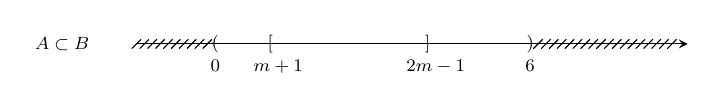
\begin{tikzpicture}[scale=1,>=stealth,font=\footnotesize,line join=round,line cap=round]
					 \draw [-stealth] (0,0)--(7,0);
					\path (1,0)  node{$($}
						 (1,-0.1) node[below]{$0$}
						(-.5,0)  node[left]{$A \subset B$};
					\path (5,0) node{$)$} 
						(5,-0.1)  node[below]{$6$};
					\path (1.7,0)  node{$[$}
						 (1.8,-0.1) node[below]{$m+1$};
					\path (3.7,0)  node{$]$}
						(3.8,-0.1) node[below]{$2m-1$}; 
					\foreach  \x in{0,0.1,...,1} \draw (\x,0)--++(45:.08)
						(\x,0)--++(-135:.08); 
					\foreach \x in{5.1,5.2,...,6.8} \draw (\x,0)--++(45:.08) 
						(\x,0)--++(-135:.08); 
				\end{tikzpicture}
		\end{center}
		Điều kiện: $m+1<2m-1 \Leftrightarrow m>2$.\\ 
		Để $A  \subset B$ thì
		 $\heva{&m+1>0\\&2m-1<6}
		\Leftrightarrow  \heva{& m>-1\\&m < \dfrac{7}{2}}
		\Leftrightarrow -1 < m < \dfrac{7}{2}$.\\ 
		Kết hợp với điều kiện ta được:  $2 < m < \dfrac{7}{2}$. Vì $m$ nguyên nên $m=3$. Vậy có $1$ giá trị $m$.
	} 
\end{bt}

% nguồn: MaHoaNH_TraLoiNgan_Lop10
\begin{bt}%[0D1V2-2]%[ma:1ac55b6e]
	Cho tập hợp $A=\left\{x;y;z\right\}$ và $B=\left\{x;y;z;t;u\right\}$. Có bao nhiêu tập $X$ thỏa  mãn $A\subset X\subset B$?
	\shortans{4} 
	 \loigiai{
		Có  $4$ tập hợp $X$ thỏa mãn $A\subset X\subset B$ là
		\[X_1=\left\{x;y;z\right\}; X_2=\left\{x;y;z;t\right\}; X_3=\left\{x;y;z;u\right\} \text{ và  } X_4=\left\{x;y;z;t;u\right\}.\]
	 }
\end{bt}

% nguồn: MaHoaNH_TraLoiNgan_Lop10
\begin{bt}%[0D1V2-2]%[ma:9dc449b7]
	Có tất cả bao nhiêu tập $X$ thỏa mãn $\left\{1;2\right\}\subset  X\subset \left\{1;2;3;4;5\right\}$?
	\shortans{8} 
	\loigiai{ 
		Các $8$ tập  $X$ thỏa mãn đề bài là
		\[\left\{1;2\right\},\left\{1;2;3\right\},\left\{1;2;4\right\},\left\{1;2;5\right\},\left\{1;2;3;4\right\},\left\{1;2;3;5\right\},\left\{1;2;4;5\right\},\left\{1;2;3;4;5\right\}.\] 
	} 
\end{bt}

% nguồn: MaHoaNH_TraLoiNgan_Lop10
\begin{bt}%[0D1V2-2]%[ma:f6953f69]
	Cho hai tập hợp khác rỗng $A=(1;5)$ và $B=(m;4m-1) \neq \varnothing$, $m \in \mathbb{R}$. Có bao nhiêu giá trị nguyên  của tham số $m$ để $B \subset A$.
	 \shortans{1}
	 \loigiai{
		Vẽ trục số thể  hiện $B \subset A$.
		\begin{center}
			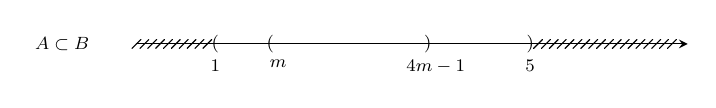
\begin{tikzpicture}[scale=1,>=stealth,font=\footnotesize,line join=round,line cap=round]
					 \draw [-stealth] (0,0)--(7,0);
					\path (1,0) node{$($} 
						(1,-0.1) node[below]{$1$} 
						 (-.5,0) node[left]{$A \subset B$};
					\path (5,0) node{$)$} 
						(5,-0.1)  node[below]{$5$};
					\path  (1.7,0) node{$($}
						(1.8,-0.1)  node[below]{$m$};
					\path (3.7,0)  node{$)$}
						 (3.8,-0.1) node[below]{$4m-1$};
					\foreach \x in{0,0.1,...,1} \draw  (\x,0)--++(45:.08)
						 (\x,0)--++(-135:.08);
					 \foreach \x in{5.1,5.2,...,6.8} \draw (\x,0)--++(45:.08)
						 (\x,0)--++(-135:.08);
				\end{tikzpicture}
		\end{center}
		Để $B \neq \varnothing $  thì $m<4 m-1 \Leftrightarrow m>\dfrac{1}{3}.~\hfill{(1)}$\\
		 Và
		$B\subset  A
		\Rightarrow \heva{&m \geq 1\\&4m-1\leq 5} 
		 \Leftrightarrow 1 \leq m \leq \dfrac{3}{2}.~\hfill{(2)}$\\
		Từ $(1)$, $(2)$ suy ra $1 \leq  m \leq \dfrac{3}{2}$.\\
		Vậy có $1$  giá trị nguyên của $m$ thì $B \subset A$.
	} 
\end{bt}

% nguồn: MaHoaNH_TraLoiNgan_Lop10
\begin{bt}%[0D1V2-2]%[ma:b9741fa3]
	Cho tập hợp $A=[4; 7]$ và $B=(2a-1; 3a+5]$ khác tập rỗng, với $a \in \mathbb{R}$. Gọi $S$  là tập hợp các giá trị nguyên của $a$ để $A \subset B$. Có bao nhiêu tập con của $S$?
	 \shortans{4}
	 \loigiai{
		\begin{itemize}
			\item Vẽ trục  số thể hiện $A \subset B$.
			\begin{center}
				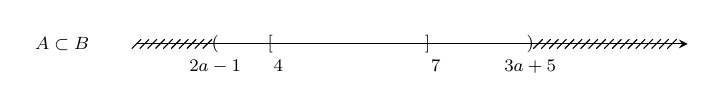
\begin{tikzpicture}[scale=1,>=stealth,font=\footnotesize,line join=round,line cap=round]
						\draw  [-stealth] (0,0)--(7,0);
						 \path (1,0) node{$($}
						(1,-0.1) node[below]{$2a-1$} 
						 (-.5,0) node[left]{$A \subset B$};
						\path (5,0) node{$)$} 
						(5,-0.1)  node[below]{$3a+5$};
						\path  (1.7,0) node{$[$}
						(1.8,-0.1)  node[below]{$4$};
						\path (3.7,0) node{$]$} 
						 (3.8,-0.1) node[below]{$7$};
						\foreach \x in{0,0.1,...,1} \draw (\x,0)--++(45:.08) 
						 (\x,0)--++(-135:.08);
						 \foreach \x in{5.1,5.2,...,6.8} \draw (\x,0)--++(45:.08)
						 (\x,0)--++(-135:.08);
					\end{tikzpicture}
			\end{center}
			\item Điều kiện tập $B$ khác tập rỗng: $2 a-1<3 a+5 \Leftrightarrow  a>-6$\, \hfill{(1)}
			\item $A \subset B \Rightarrow \heva{& 2a-1<4 \\& 3a+5 \geqslant 7 } \Leftrightarrow \heva{& a<\dfrac{5}{2} \\& a \geqslant  \dfrac{2}{3}} \Leftrightarrow \dfrac{2}{3} \leqslant a<\dfrac{5}{2}.$ \, \hfill{(2)}
			\item Kết hợp $(1)$  và $(2)$, ta được $\dfrac{2}{3} \leqslant a<\dfrac{5}{2}$.
			\item  Xét các giá trị $a \in \mathbb{Z} \Rightarrow S=\{1; 2\}$.
			\item Có $4$ tập con của $S$ là $\varnothing $; $\{1\} $; $\{2\}$ và $S=\{1;  2\}$.
		\end{itemize}
	} 
\end{bt}

% nguồn: MaHoaNH_TraLoiNgan_Lop10
\begin{bt}%[0D1V2-2]%[ma:8c3a2e78]
	Lớp $10$A có $10$ học sinh giỏi Toán, $10$ học sinh giỏi Lý, $11$ học sinh giỏi hóa, $6$ học sinh giỏi cả Toán và Lý, $5$ học sinh giỏi cả Hóa và Lý, $4$ học sinh giỏi cả Toán và Hóa, $3$ học sinh giỏi cả ba môn Toán, Lý,  Hóa. Tính học sinh giỏi ít nhất một trong ba môn (Toán, Lý, Hóa) của lớp $10$A?
	 \shortans{18}
	\loigiai{ 
		Theo giả thiết đề bài cho, ta có  biểu đồ Ven
		\begin{center}
			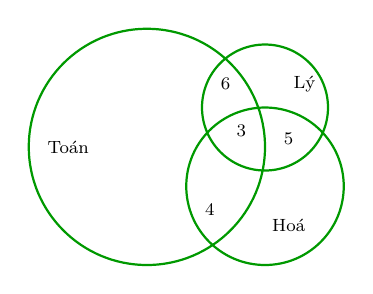
\begin{tikzpicture}[>=stealth,line join=round,line cap=round,font=\footnotesize,scale=1]
					\draw [thick,green!60!black] (0,0) circle (1.5) 
						(1.5,-0.5)  circle (1)
						(1.5,0.5) circle  (0.8);
					\draw (1,.8) node {$6$} 
						 (1.2,.2) node {$3$}
						(2,.8) node {Lý} 
						 (1.8,.1) node {$5$}
						(1.8,-1)  node {Hoá}
						(.8,-.8)  node {$4$}
						(-1,0) node  {Toán};
				\end{tikzpicture}
		\end{center}
		Dựa vào biểu đồ Ven, ta có học sinh giỏi ít nhất một trong ba môn (Toán, Lý, Hóa)  của lớp $10$A là
		\begin{itemize}
			\item Số học  sinh giỏi Toán $6+4+3=13$.
			\item Số học sinh  giỏi Lý $6+5+3=14$.
			\item Số học  sinh giỏi Hóa $4+5+3=12$.
		\end{itemize}
		Ta lại có 
		\begin{itemize}
			\item Số học  sinh giỏi cả Toán và Lý $6$.
			\item Số học sinh giỏi cả Toán và Hóa $4$. 
			\item Số học sinh giỏi cả Hóa  và Lý $5$.
			\item Và số học  sinh giỏi cả Toán, Lý và Hóa là $3$.
			\item Số học sinh giỏi hơn một môn  là $4+6+5+3=18$.
		\end{itemize}
	 }
\end{bt}


%%%%%%%%%%%%%%%% TỰ LUẬN %%%%%%%%%%%%%%%%

% nguồn: MaHoaNH_TuLuan_Lop10
\begin{bt}%[0D1H2-2]%[ma:bfb71ee8]
	Cho tập hợp $A=(2;+\infty)$ và tập hợp $B=(m;+\infty)$. Tìm điều kiện cần và  đủ của $m$ để $B$ là tập con của $A$?
	\loigiai{Ta có  $B\subset A$ khi và chỉ khi $\forall x\in B\Rightarrow x\in A$ $\Rightarrow m\ge 2$.
	 }
\end{bt}

% nguồn: MaHoaNH_TuLuan_Lop10
\begin{bt}%[0D1H2-2]%[ma:a1f9a875]
	Cho  hai tập hợp $A=\left[1;3\right]$ và $B=\left[m;m+1\right]$. Tìm tất cả giá trị của tham số $m$ để $B\subset A$.
	\loigiai{Ta có $B\subset A\Leftrightarrow \heva{&m\ge  1\\&m+1\le 3} \Leftrightarrow \heva{&m\ge 1\\&m\le 2.}$\\
		Vậy $1\le m\le 2$. 
	 }
\end{bt}

% nguồn: MaHoaNH_TuLuan_Lop10
\begin{bt}%[0D1H2-2]%[ma:7a14d165]
	Cho tập hợp $A = \left\{x \in \mathbb{Z} \mid \dfrac{x^2  + 2}{x} \in \mathbb{Z}\right\}$.
	\begin{enumerate}
		\item Hãy xác định tập $A$ bằng cách liệt  kê các phần tử.
		\item Tìm tất cả các tập con của tập hợp  $A$ mà số phần tử của nó nhỏ hơn $3$.
	\end{enumerate}
	\loigiai{ 
		\begin{enumerate}
			\item Ta có $\dfrac{x^2 + 2}{x} = x + \dfrac{2}{x} \in \mathbb{Z}$ (với $ x \in \mathbb{Z}$) khi và chỉ khi $x$ là ước của $2$ hay \begin{center}
				$x  \in \{-2; -1; 1; 2\}$.
			\end{center}
			Vậy $A = \{-2; -1;  1; 2\}$.
			\item  Tất cả các tập con của tập hợp $A$ mà số phần tử của nó nhỏ hơn $3$ là\\
			 Tập không có phần tử nào $\varnothing$.\\
			Tập có một  phần tử là $\{-2\}$, $\{-1\}$, $\{1\}$, $\{2\}$.\\
			Tập có hai phần tử là $\{-2; -1\}$, $\{-2; 1\}$, $\{-2;  2\}$, $\{-1; 1\}$, $\{-1; 2\}$, $\{1; 2\}$.
		\end{enumerate}
	} 
\end{bt}

% nguồn: MaHoaNH_TuLuan_Lop10
\begin{bt}%[0D1H2-2]%[ma:3240b329]
	 Tìm tất cả các tập con, các tập con gồm hai phần tử của các tập hợp sau
	\begin{multicols}{2}
		\begin{enumerate}
			\item  $A=\left\{1;2\right\}$;
			 \item $B=\left\{1;2;3\right\}$;
			\item $C=\left\{a;b;c\right\}$; 
			\item $D=\left\{x\in \mathbb{R}\mid 2x^2-5x+2=0\right\}$. 
		\end{enumerate}
	\end{multicols}
	\loigiai{\begin{enumerate}
		\item Tập $A$ có các tập con gồm $2$ phần tử  là $\left\{1;2\right\}$
		\item Tập $B$ có các tập con gồm $2$ phần tử là  $\left\{1,2\right\}$; $\left\{2,3\right\}$; $\left\{1,3\right\}$.
		 \item Tập $C$ có các tập con gồm $2$ phần tử là $\left\{a;b\right\}$; $\left\{a;c\right\}$; $\left\{a;d\right\}$; $\left\{b;c\right\}$; $\left\{b;d\right\}$; $\left\{c;d\right\}$.
		\item  $x^2-4x+2=0\Leftrightarrow \hoac{&x_1=2\\
		&x_2=\dfrac{1}{2}}$ suy  ra $D=\left\{\dfrac{1}{2};2\right\}$.\\
		Tập  con của nó chính là nó vì $D$ chỉ có đúng $2$ phần tử.
	\end{enumerate}
 }
\end{bt}

% nguồn: MaHoaNH_TuLuan_Lop10
\begin{bt}%[0D1H2-2]%[ma:557c14c7]
	 Cho $A=\left\{-4;-2;-1;2;3;4\right\}$ và $B=\left\{x\in \mathbb{Z}\mid \left|x\right|\le 4\right\}$. Tìm tập hợp $X$ sao cho
	\begin{enumerate}
		\item $A\subset X\subset  B$;
		\item $A\cup X=B$ với $X$ có  đúng bốn phần tử.
	\end{enumerate}
	\loigiai{\begin{enumerate}
		\item Ta có  $\heva{&\left|x\right|\le 4\\&x\in \mathbb{Z}} \Leftrightarrow \heva{&-4\le x\le 4\\
		&x\in \mathbb{Z}} \Leftrightarrow  x\in \left\{-4;-3;-2;-1;0;1;2;3;4\right\}$.\\
		Suy ra $B=\left\{-4;-3;-2;-1;0;1;2;3;4\right\}$. 
		\item Ta có $\left\{-4;-2;-1;2;3;4\right\}\subset X\subset \left\{-4;-3;-2;-1;0;1;2;3;4\right\}$ suy ra  tập hợp $X$ là
		 \begin{center}
		 	 $\left\{-4;-2;-1;2;3;4\right\}$, $\left\{-4;-2;-3;-1;2;3;4\right\}$,\\
		 	$\left\{-4;-2;-1;0;2;3;4\right\}$, $\left\{-4;-2;-1;1;2;3;4\right\}$,\\ 
		 	$\left\{-4;-2;-3;-1;0;2;3;4\right\}$, $\left\{-4;-2;-3;-1;1;2;3;4\right\}$,  \\
		 	$\left\{-4;-2;-1;0;1;2;3;4\right\}$, $\left\{-4;-3;-2;-1;0;1;2;3;4\right\}$. 
		 \end{center}
		\item Ta có $A\cup X=B$ với $X$ có đúng bốn  phần tử khi đó tập hợp $X$ là $\left\{-4;-3;0;1\right\}$, $\left\{-3;-2;0;1\right\}$, $\left\{-3;-1;0;1\right\}$, $\left\{-3;0;1;2\right\}$, $\left\{-3;0;1;3\right\}$, $\left\{-3;0;1;4\right\}$.
	\end{enumerate}
	} 
\end{bt}

% nguồn: MaHoaNH_TuLuan_Lop10
\begin{bt}%[0D1V2-2]%[ma:dfcb99f9]
	Cho $A=\left[m-3; \dfrac{m+2}{4}\right)$, $B=(-\infty;-1) \cup [2;+\infty)$. Xác định $m$ để  ${A \cap B=\varnothing}$.
	 \loigiai{ Ta có
		\[ 
		A  \cap B = \varnothing
		\Leftrightarrow \heva{&m-3  < \dfrac{m+2}{4}\\&m-3 \geq -1\\&\dfrac{m+2}{4} \leq 2}
		\Leftrightarrow \heva{&m<\dfrac{14}{3}\\&m \geq 2\\&m \leq 6} 
		\Leftrightarrow  2 \leq m < \dfrac{14}{3}.
		 \]
	} 
\end{bt}

% nguồn: MaHoaNH_TuLuan_Lop10
\begin{bt}%[0D1V2-2]%[ma:1a0d2a41]
	Cho $2$ tập khác rỗng $A=(m-1; 4]$;  $B=(-2; 2 m+2)$, $m \in \mathbb{R}$. Tìm $m$ nguyên dương để $A \subset B$.
	 \loigiai{
		Vẽ trục số thể hiện $A \subset B$. 
		\begin{center}
			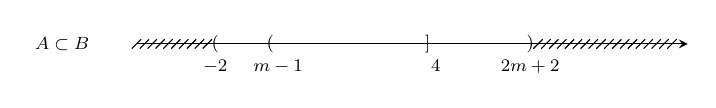
\begin{tikzpicture}[scale=1,>=stealth,font=\footnotesize,line join=round,line cap=round]
					\draw [-stealth] (0,0)--(7,0); 
					\path (1,0) node{$($} 
						(1,-0.1)  node[below]{$-2$}
						 (-.5,0) node[left]{$A \subset B$};
					\path (5,0)  node{$)$}
						(5,-0.1)  node[below]{$2m+2$};
					\path (1.7,0) node{$($} 
						(1.8,-0.1) node[below]{$m-1$}; 
					\path  (3.7,0) node{$]$}
						(3.8,-0.1)  node[below]{$4$};
					\foreach \x in{0,0.1,...,1} \draw  (\x,0)--++(45:.08)
						(\x,0)--++(-135:.08); 
					\foreach \x  in{5.1,5.2,...,6.8} \draw (\x,0)--++(45:.08)
						(\x,0)--++(-135:.08); 
				\end{tikzpicture}
		\end{center}
		Với $2$ tập khác rỗng $A$, $B$ ta có điều kiện $  \heva{&m-1<4 \\&2m+2>-2}
		\Leftrightarrow  \heva{&m<5\\&m>-2}
		\Leftrightarrow-2<m<5$.\\ 
		 Để $A \subset B
		\Leftrightarrow \heva{& m-1 \geqslant-2 \\& 2  m+2>4}
		\Leftrightarrow \heva{& m  \geqslant-1 \\& 2 m+2>4}
		 \Leftrightarrow \heva{& m \geqslant-1 \\& m>1}
		\Leftrightarrow  m>1$.\\
		So với điều kiện $\Rightarrow 1<m<5$. Do  đó có $3$ giá trị nguyên của $m$ thỏa mãn $A \subset B$.
	 }
\end{bt}

% nguồn: MaHoaNH_TuLuan_Lop10
\begin{bt}%[0D1B2-2]%[ma:4094ec57]
	Cho tập hợp $A = \{1;2\}$, $B =  \{0;1;2;3\}$. Tìm tất cả tập $X$ thỏa mãn $A \subset X \subset B$.
	 \loigiai{
		Các tập hợp $X$ thỏa mãn $A  \subset X \subset B$ là $\{1;2\}$, $\{1;2;0\}$, $\{1;2;3\}$, $\{0;1;2;3\}$.
	 }
\end{bt}

% nguồn: MaHoaNH_TuLuan_Lop10
\begin{bt}%[CTST10]%[0D1B2-2]%[ma:6458b74e]
	Hãy viết tất cả các tập con của tập hợp $ B=\{0;1;2\} $. 
	 \loigiai{
		Các tập con của tập hợp $ B=\{0;1;2\} $ là $ \varnothing $, $ \{0\} $, $ \{1\} $, $ \{2\} $, $ \{0;1\} $, $ \{0;2\} $, $ \{1;2\} $, $  \{0;1;2\} $.
	} 
\end{bt}

% nguồn: MaHoaNH_TuLuan_Lop10
\begin{bt}%[0D1B2-2]%[ma:78788352]
	Cho tập $A= \left\{ a;b;c \right\} $. Tìm tất cả các  tập con của $A$.
	 \loigiai{
		Theo tính chất về tập hợp  con, ta có $\varnothing \subset A,~A \subset A$. Ngoài ra, còn có các tập hợp con sau:\\
		$\bullet$ Tập hợp con  có $1$ phần tử gồm có $\left\{ a \right\}$, $\left\{ b \right\}$, $\left\{ c \right\}$.\\
		$\bullet$ Tập  hợp con có $2$ phần tử gồm có $\left\{ a;b \right\}$, $\left\{ b;c \right\}$, $\left\{ a;c \right\}$.\\
		\underline{Nhận xét}: Nếu một tập hợp có $n$ phần tử (với $n \in  \mathbb{N}^*$) thì số tập con của nó là $2^n$.
	 }
\end{bt}

% nguồn: MaHoaNH_TuLuan_Lop10
\begin{bt}%[0D1K2-2]%[ma:2725a98d]
	Cho $A=\{2;5\}, B=\{5;x\}, C=\{x;y;5\}$. Tìm các cặp số $\{x;y\}$  để $A=B=C$.
	 \loigiai{
		Vì $A=B=C$ nên cả $3$ tập hợp $A$, $B$, $C$ chỉ chứa $2$ phần tử là $2$ và $5$.\\ 
		Do đó ta có $\left\{\begin{aligned}
		&x=2\\ 
		&\left[\begin{aligned}
		&y=2\\ 
		&y=5.\\ 
	\end{aligned}\right.\\
	\end{aligned}\right.$
	 }
\end{bt}

% nguồn: MaHoaNH_TuLuan_Lop10
\begin{bt}%[CTST10]%[0D1B2-2]%[ma:81ec1bc9]
	Trong mỗi cặp  tập hợp sau đây, tập hợp nào là tập con của tập còn lại? Chúng có bằng nhau không?
	\begin{enumerate}[a)]
		\item $ A=\left\{x\in \mathbb{N}\ \mid dle| \ x<2\right\} $ và $ B=\left\{x\in  \mathbb{R}\ \mid dle| \ x^2-x=0\right\} $;
		\item  $ C $ là tập hợp các hình thoi và $ D $ là tập hợp các hình vuông;
		 \item $ E=(-1;1] $ và $ F=(-\infty;2] $.
	\end{enumerate}
	\loigiai{ 
		\begin{enumerate}[a)]
			\item Ta có $ A=\left\{x\in \mathbb{N}\ \mid dle| \ x<2\right\} =\left\{0;1 \right\} $ và $ B=\left\{x\in \mathbb{R}\ \mid dle| \  x^2-x=0\right\} =\left\{0;1 \right\} $. Do đó $ A=B $.
			\item $ C $ là tập hợp các hình thoi và $ D $ là tập hợp các  hình vuông.\\
			Ta có hình vuông là hình thoi có bốn góc vuông. Do đó  $ D \subset C $, $ D $ khác $ C $.
			\item $ E=(-1;1] $ và $ F=(-\infty;2] $. Ta có $ E\subset  F $, $ E $ khác $ F $.
		\end{enumerate}
	 }
\end{bt}

% nguồn: MaHoaNH_TuLuan_Lop10
\begin{bt}%[0D1K2-2]%[ma:e2e8e99e]
	Tìm tất cả các tập con, các tập con gồm hai phần tử của các  tập hợp sau:
	\begin{enumerate}
		\item  $A=\left\{{1;2}\right\}$.
		\item $B=\left\{{1;2;3}\right\}$. 
		 \item $C=\left\{{x\in \mathbb{R}\left|{2x^2-5x+2=0}\right.}\right\}$.
		\item $D=\left\{{x\in \mathbb{Q}\left|{x^2-4x+2=0}\right.}\right\}$. 
	\end{enumerate}
	\loigiai{ 
		\begin{enumerate}
			 \item Tập con gồm $\varnothing$, $\{1\}$, $\{2\}$, $\{1;2\}$
			\item Tập con gồm $\varnothing$, $\{1\}$, $\{2\}$, $\{3\}$, $\{1;2\}$, $\{1;3\}$,  $\{2;3\}$, $\{1;2;3\}$
			\item Ta  có $2x^2-5x+2=0\Leftrightarrow \hoac{&x=\dfrac{1}{2}\in \mathbb{R}\\&x=2\in \mathbb{R}}\Rightarrow C=\left\{\dfrac{1}{2};2\right\}$. Suy ra tập con gồm $\varnothing$, $\{2\}$, $\left\{\dfrac{1}{2}\right\}$, $\left\{2;\dfrac{1}{2}\right\}$
			\item Ta có $x^2-4x+2=0\Leftrightarrow x=2\pm \sqrt{2}\notin \mathbb{Q}\Rightarrow D=\varnothing$. 
		\end{enumerate}
	} 
\end{bt}

% nguồn: MaHoaNH_TuLuan_Lop10
\begin{bt}%[0D1K2-2]%[ma:0dbd2da3]
	Trong các tập hợp sau,  tập nào là tập con của tập nào?
	\begin{enumerate}
		\item $A=\left\{{1;2;3}\right\}$, $B=\left\{{x\in  \mathbb{N}\left|{x<4}\right.}\right\}$, $C=\left(0;+\infty\right)$, $D=\left\{{x\in \mathbb{R}\left|{2x^2-7x+3=0}\right.}\right\}$.
		\item $A=$ Tập các ước số tự nhiên của $6$; $B=$ Tập các ước số tự nhiên của  $12$.
		\item $A=$ Tập các hình bình hành; $B=$ Tập các  hình chữ nhật;
		$C=$ Tập các hình thoi; $D=$ Tập các hình  vuông.
		\item $A=$ Tập các tam  giác cân; $B=$ Tập các tam giác đều;
		$C=$ Tập các tam giác vuông; $D=$ Tập  các tam giác vuông cân.
	\end{enumerate}
	\loigiai{ 
		\begin{enumerate}
			\item  $B=\{0;1;2;3\}$, $D=\left\{\dfrac{1}{2};3\right\}$. Suy ra $A\subset B\subset C$, $D\subset C$.
			\item $A=\{1;2;3;6\}$,  $B=\{1;2;3;4;6;12\}$. Suy ra $A\subset B$.
			\item Dựa theo tính chất hình vuông, hình chữ nhật, hình thoi, hình bình hành. Ta có $D\subset  C\subset A$, $D\subset B\subset A$.
			\item Dựa theo tính chất  tam giác vuông, vuông cân, cân, đều. Ta có $B\subset A$, $D\subset C$, $D\subset A$.
		\end{enumerate}
	} 
\end{bt}

% nguồn: MaHoaNH_TuLuan_Lop10
\begin{bt}%[0D1K2-2]%[ma:8dec1109]
	Cho  tập hợp $M=\{-2;-1;0;1;2;3;4;5\}$.
	\begin{enumerate}
		\item Tìm tất cả  tập hợp con có $1$ phần tử của tập $M$.
		\item Tìm tất cả tập hợp con có $2$ phần  tử của tập $M$.
		\item  Tập $M$ có tất cả bao nhiêu tập hợp con?
		\item Tập $M$ có tất cả bao nhiêu tập hợp con có ít  nhất $1$ phần tử?
		\item Tập $M$ có tất  cả bao nhiêu tập hợp con khác $M$?
	\end{enumerate}
	\loigiai{ 
	\begin{enumerate}
		\item Tất cả  tập con có $1$ phần tử của $M$ là $\{-2\}$, $\{-1\}$, $\{0\}$, $\{1\}$, $\{2\}$, $\{3\}$, $\{4\}$, $\{5\}$.
		\item Tất cả tập con có $2$ phần tử của $M$ là $\{-2;-1\}$, $\{-2;0\}$, $\{-2;1\}$, $\{-2;2\}$, $\{-2;3\}$, $\{-2;4\}$, $\{-2;5\}$, $\{-1;0\}$, $\{-1;1\}$, $\{-1;2\}$,  $\{-1;3\}$, $\{-1;4\}$, $\{-1;5\}$, $\{0;1\}$, $\{0;2\}$, $\{0;3\}$, $\{0;4\}$, $\{0;5\}$, $\{1;2\}$, $\{1;3\}$, $\{1;4\}$, $\{1;5\}$, $\{2;3\}$, $\{2;4\}$, $\{2;5\}$, $\{3;4\}$, $\{3;5\}$, $\{4;5\}$.
		\item Tập hợp $M$ có $8$ phần  tử. Số tập hợp con của $M$ là $2^8=256$.
		\item Tập  con không có phần tử của $M$ là $\varnothing$.\\
		Số tập hợp con có ít nhất $1$ phần tử của $M$ là  $2^8-1=255$.
		\item  Số tập hợp con khác $M$ là $2^8-1=255$.
	\end{enumerate}
	} 
\end{bt}
